\documentclass{article}
\usepackage{amsmath, amsthm, amssymb, graphicx, enumitem, esvect}
\usepackage[english]{babel}
\usepackage[letterpaper,top=2cm,bottom=2cm,left=3cm,right=3cm,marginparwidth=1.75cm]{geometry}
\usepackage[most]{tcolorbox}
\usepackage{hyperref}
\usepackage{graphicx}



\newcommand{\bookBegin}[1]{\begin{tcolorbox}[colback=black!5!white,colframe=black!75!black,title={\textit{Operating Systems, Three Easy Pieces: #1}}]}
  \newcommand{\bookEnd}{\end{tcolorbox}}

\newcommand{\definitionBegin}[1]{\begin{tcolorbox}[title={Definition: #1}]}
  \newcommand{\definitionEnd}{\end{tcolorbox}}

\newcommand{\exampleBegin}[1]{\begin{tcolorbox}[colback=blue!5!white,colframe=black!75!blue,title={Example:
      #1}]}
  \newcommand{\exampleEnd}{\end{tcolorbox}}

\newcommand{\abstractionBegin}[1]{\begin{tcolorbox}[colback=violet!5!white,colframe=violet,title={Abstraction:
      #1}]}
  \newcommand{\abstractionEnd}{\end{tcolorbox}}

\newcommand{\refto}[2]{\textbf{\ref{#1:#2} \nameref{#1:#2}}}

\title{CS 111}
% \author{Warren Kim}
\date{}

\begin{document}
\maketitle

\tableofcontents
\newpage

\section*{Preface: Legend}
\begin{tcolorbox}[colback=black!5!white,colframe=black!75!black,title=\textit{Operating Systems, Three Easy Pieces}]
  Text in these boxes will indicate that further details can be found in the textbook
  (\textit{Operating Systems: Three Easy Pieces} by Arpaci-Dusseau)
\end{tcolorbox}

\begin{tcolorbox}[title=Definitions]
  Any definitions will be appear in a grey box like this one. There may be more than one definition
  per box if the topics are dependent on each other or are closely related.
\end{tcolorbox}

\begin{tcolorbox}[colback=blue!5!white,colframe=black!75!blue,title=Examples]
  Any examples will be appear in a blue box like this one. Examples will typically showcase a scenario
  that emphasizes the importance of a particular topic.
\end{tcolorbox}

\begin{tcolorbox}[colback=violet!5!white,colframe=violet,title=Abstractions] 
  Layers of abstractions will appear in a violet box like this one. The key point of this box is to
  actively reinforce the concept of abstraction (and recognize how important it is in computer science!).
\end{tcolorbox}





\section*{Preface: Introduction to Abstraction}
\begin{tcolorbox}[title=Definition: Abstraction]
  \textbf{Abstraction} is the concept of providing a (relatively) simple interface to higher level
  programs, hiding unnecessary complexity.
\end{tcolorbox}

The OS implements these abstract resources using physical resources, and thus is the source of one
of the main dilemmas of OS design: What should you abstract?

\begin{tcolorbox}[colback=blue!5!white,colframe=black!75!blue,title=Example: Network Neverland]
  Network cards consist of intricate technical details and specifications, but most users don't care
  about them. As a result, the operating system abstracts the technical aspects of a
  specific network card, such as the process of sending a message, for higher-level programs. Instead
  of manually performing each step to send a message using a particular network card, users can simply
  call the OS's \texttt{send()}\footnote{The actual function name may vary.} function and let the
  operating system handle the complex operations. 
\end{tcolorbox}


\subsection*{Why Abstract?}
Abstraction is utilized to simplify code development and comprehension for programmers and
users. Furthermore, it naturally fosters a highly modular codebase as each abstraction introduces an
additional layer of modularity. Moreover, by concealing complexity at each layer of abstraction, it
encourages programmers to concentrate on the essential functionality of a component. 

Due to variability of a machine's hardware and software, we can abstract the common
functionality and make different types appear the same. This way, applications only need to
interface with a common library. 





\section{Overview}
This section defines what an operating system is as well as gives motivating reasons as to why we
should be studying them. 


\subsection{What is an Operating System?}
\begin{tcolorbox}[title=Definition: Operating System]
  An \textbf{operating system (OS)} is system software that acts as an intermediary between hardware and
  higher level applications (e.g. higher level system software, user processes), acting as an
  intermediary between the two. It manages hardware and software resources and provides common
  services for user programs. 
\end{tcolorbox}

\begin{tcolorbox}[colback=violet!5!white,colframe=violet,title=Abstraction: The Operating System] 
  The operating system plays a crucial role in managing hardware resources for programs, ensuring
  controlled sharing, privacy, and overseeing their execution. Moreover, it provides a layer of
  abstraction that enhances software portability. 
\end{tcolorbox}


\subsection{Why Study Them?}
We study operating systems because we rely on the \textit{\textbf{services}} they offer.

\begin{tcolorbox}[title=Definition: Services]
  In the context of operating systems, \textbf{services} are functionality that is provided
  for by the operating system. They can be accessed via the operating system's API in the form of
  system calls. 
\end{tcolorbox}

Moreover, a lot of hard problems that we run into at the application layer have (probably) already
been solved in the context of operating systems !

\begin{tcolorbox}[colback=blue!5!white,colframe=black!75!blue,title=Example: Difficult Downloads]
  Suppose you are developing a web browser and implementing a \textit{download} feature. While
  downloading things one by one works fine, what if you need to download multiple items from different
  sites simultaneously? Thinking abstractly, we can see that this is a problem of coordinating
  concurrent activities, and fortunately, this problem has already been solved in the context of
  operating systems! Since you have already learned how to tackle this issue in operating systems, now
  you can apply the same solution to your \textit{download} problem!
\end{tcolorbox}


\subsection{Key Topics (OS Wisdom)}
When thinking of how to solve complex problems, these are some things you should take into
consideration (to hopefully make your life a lot easier).


\subsubsection*{Objects and Operations}
Think of a service as an object with a set of well-defined operations. Moreover, thinking of the
underlying data structure(s) of an object may be useful in many situations.  


\subsubsection*{Interface v. Implementation}
\begin{tcolorbox}[title=Definition: Interface and Implementation]
  An \textbf{interface} defines the collection of functionalities offered by your software. It
  specifies the method names, signatures, and the \textit{purpose} of each component. 
  \tcblower
  An \textbf{implementation} refers to the actual code that provides the functionality described by
  the interface. It specifies \textit{how} the interface's operations are executed and realized in practice. 
\end{tcolorbox}
We separate the two components to improve modularity and create robust, well-structured code. It
allows for different compliant implementations (as long as they adhere to the agreed-upon interface
specifications). This provides immense flexibility at the implementation level!

\begin{tcolorbox}[colback=blue!5!white,colframe=black!75!blue,title=Example: Sort Swapping]
  Assume you are writing a library that contains a collection of common algorithms, one of them
  being \texttt{sort()}. Being the genius that you are, your implementation is as follows: Randomly
  reorder the elements until they're sorted. By some miracle, your library garners a lot of
  attention, but users are complaining that \texttt{sort()} takes too long. Not knowing what's wrong
  with your implementation, you take DSA\footnote[1]{DSA: Data Structures and Algorithms} 
  and learn that you've got shit for brains. You want to rewrite \texttt{sort()} but are worried
  that it might break the interface. However, you remember that interface $\neq$ implementation, so
  you rewrite \texttt{sort()} (using something like merge sort) pushing this new implementation
  into production, and bragging about how \texttt{sort()} now runs in O($n \log n$) time. 
\end{tcolorbox}

\subsubsection*{Encapsulation}
We want to abstract away complexity (when appropriate) into an interface for ease of use.

\subsubsection*{Policy and Mechanism}
\label{subsubsec:PAM}
\begin{tcolorbox}[title=Definition: Policy and Mechanism]
  A \textbf{policy} is a high-level rule or guideline that governs the \textit{behavior} of a
  system.
  \tcblower
  A \textbf{mechanism} is the implementation that is used to \textit{enforce} the policy.
\end{tcolorbox}
It is important to note that keeping policy and mechanism independent of one another is crucial. By
separating policies from the underlying mechanisms, it becomes easier to change or modify policies
without affecting the core functionality or technical implementation. This approach provides the
ability to update policies independently from the underlying mechanisms, promoting modifiability,
maintainability, and customization when designing software.


\subsection{Why is the OS Special?}
\begin{tcolorbox}[title=Definition: Standard and Privileged Instruction Set]
  The \textbf{standard instruction set} is the set of hardware instructions that can be executed by anybody.
  \tcblower
  The \textbf{privilaged instruction set} is the set of hardware instructions only the kernel can
  execute. When an application wants to execute a privilaged instruction, it must ask the kernel to
  execute it for them.
\end{tcolorbox}

The OS is special for a number of reasons. Mainly, it has \textit{complete} access to the privileged
instruction set, \textit{all} of memory and I/O, and mediates applications' access to
hardware. This implies that the OS is \textit{trusted} to always act in good faith. Thus, the OS
stays up and running as long as the machine is still powered on (theoretically), and if the OS crashes,
you're fucked lol.


\subsection{Miscellaneous}
Below are a list of miscellaneous topics.
\subsubsection{Definitions}
\begin{tcolorbox}[title=Definition: Instruction Set Architectures]
  An \textbf{instruction set architecture (ISA)} is the set of instructions supported by a
  computers. There are multiple (all incompatible) ISA's and they usually come in families.
\end{tcolorbox}

ISA's usually come with privilaged and standard instruction sets.

\begin{tcolorbox}[title=Definition: Platform]
  A \textbf{platform} is the combination of hardware and software that provide an environment for
  running applications.
\end{tcolorbox}

Common platforms include: Windows, [Mac, i]OS, Linux.

\begin{tcolorbox}[title=Definition: Binary Distribution Model]
  The \textbf{binary distribution model} is the paradigm of distributing software in compiled or
  machine code in the form of executables.
\end{tcolorbox}

The binary distribution model is good for performance and security, but lacks in flexibility and is
dependent on the platform you compile it for.

\begin{tcolorbox}[title=Definition: Portability]
  \textbf{Portability} refers to the ability to be adapted to different platforms with minimal
  modifications to the source code.
\end{tcolorbox}

Portability is important if you're an OS designer because you want to maximize the number of people
using your product $\implies$ your OS should run on many ISA's and make minimal assumptions about
specific hardware.





% \begin{tcolorbox}[colback=red!5!white,colframe=red!75!red,title=WIP]
%   \subsection{Virtualization}
%   \begin{tcolorbox}[colback=black!5!white,colframe=black!75!black,title=\textit{4) The Abstraction: The Process}]
%     \begin{tcolorbox}[title=Definition: Process]
%       A \textbf{process} is an abstraction of a running program. It has an API 
%     \end{tcolorbox}
%   \end{tcolorbox}
% \end{tcolorbox}



\section{Resource Types}
This section covers three types of OS resources: serially reusable, partitionable, and
sharable.

\begin{tcolorbox}[title=Definition: Graceful Transition]
  A \textbf{graceful transitions} refers to the process of transferring control between two jobs
  such that there are no resource conflicts. 
\end{tcolorbox}

A graceful transition maintains system stability, data integrity and therefore cleanly releases
resources. They typically ensure that users leave resources in a clean state; i.e. each
subsequent user finds the resource in a ``like new'' condition.


\subsection{Serially Reusable}
\begin{tcolorbox}[title=Definition: Serially Reusable Resource]
  \textbf{Serially reusable resources} are resources that can be used by a single process at a time
  (sequentially) and are not designed to be shared in parallel.
\end{tcolorbox}

These resources require access control mechanisms to ensure that only one process can access them at
any given time. This control ensures a graceful transition between users and prevents conflicts or
data corruption that may arise from concurrent access.

\begin{tcolorbox}[colback=blue!5!white,colframe=black!75!blue,title=Example: Printing Process]
  Printers are a serially reusable resource: multiple job can use it but only a single job will be
  printed at a time. 
\end{tcolorbox}

\subsection{Partitionable}
\begin{tcolorbox}[title=Definition: Partitionable Resource]
  \textbf{Partitionable resources} can be divided up (or \textit{partitioned}) into smaller,
  disjoint\footnote{Disjoint: Independent of one another.} segments.  
\end{tcolorbox}

These resources require access control mechanisms to ensure that each segment is
\textit{contained}\footnote{Contained: Resources outside of a partition are not accessible.} and
\textit{private}\footnote{Private: External users cannot access the resources in your
  partition.}. Partitionable resources can be temporarily allocated (e.g. RAM, CPU \textit{time
  slice}, etc.) or permanently allocated (e.g. Disk
storage\footnote{Disk storage is permanently allocated until it isn't. You can use something like
  \texttt{fdisk} (in Linux) to modify partitions.}, database tables, etc.).

\begin{tcolorbox}[colback=blue!5!white,colframe=black!75!blue,title=Example: Memory Mania and Disk Division]
  Memory can be partitioned, allowing multiple unique processes to access their own allocated memory
  space independently.
  \tcblower
  Disk storage can be partitioned into separate logical volumes! This is commonly used to dual-boot
  different operating systems. Recently, M1(/2\textit{ish}) Apple products can now run Linux on
  bare metal (still in beta !) via Asahi Linux!
\end{tcolorbox}

Graceful transitions are still necessary in partitionable resources! Partitionable resources that
aren't permanently allocated need to clean up after themselves.


\subsection{Shareable}

\begin{tcolorbox}[title=Definition: Shareable Resource]
  \textbf{Shareable resources} are usable by multiple \textit{concurrent} clients. They need not
  ``wait'' for access nor do they ``own'' a particular subset of a given shared resource. 
\end{tcolorbox}

These resources require access control mechanisms to ensure that the shareable resource is used in a
controlled and secured manner.

\begin{tcolorbox}[colback=blue!5!white,colframe=black!75!blue,title=Example: Cloud Crazy] 
  The cloud (e.g. Google Drive, Oracle Cloud, etc.) is a powerful shared resource! It enables
  multiple concurrent users to access shared folders and files, facilitating simultaneous editing
  and collaboration.
\end{tcolorbox}

Graceful transitions typically are not necessary since a shareable resource generally doesn't change
state \textit{or} doesn't require any clean up. In the example above, while the cloud files change
state, there is no cleaning up to do, so a graceful transition is not necessary (what's clean
doesn't need cleaning).





\section{Services}
The OS provides services in a multitude of ways. This section will introduce and explain how
services are provided throughout the software stack.


\subsection{Subroutines}
\begin{tcolorbox}[title=Definition: Subroutine]
  A \textbf{subroutine} in the context of operating systems is a small, self-contained and reusable
  portion of code that performs a specific function.
\end{tcolorbox}

Subroutines are usually called directly, and operate like normal code (stack manipulation), and are
typically seen in higher layers of the OS stack. They are fast, but usually cannot use the
privileged instruction set. Furthermore, they are usually not language agnostic. The most common way
to implement these subroutines are libraries!

\subsection{Libraries}
One way the OS provides services to users is via libraries. Standard utility functions such as
\texttt{malloc} can be found in libraries (in this case, \texttt{stdlib.h}). So what exactly is a
library?

\begin{tcolorbox}[title=Definition: Library]
  A \textbf{library} is a collection of code modules that encapsulate common operations, algorithms,
  and functionality. 
\end{tcolorbox}

\begin{tcolorbox}[colback=violet!5!white,colframe=violet,title=Abstraction: Libraries] 
  Most systems are equipped with a wide range of standard libraries, which are designed to be
  reused. These libraries encapsulate complexity and provide an additional layer of abstraction,
  simplifying problem-solving. 
\end{tcolorbox}

\begin{tcolorbox}[colback=blue!5!white,colframe=black!75!blue,title=Example: DSA Doozy] 
  In DSA, you likely had to implement different types of data structures (linear, hierarchical,
  graphical, etc.) and algorithms (search, divide/conquer, dynamic programming). Imagine your
  surprise when you find out most of these data structures and algorithms have already been written
  (and probably perform better than your implementation, no offense).
\end{tcolorbox}

\subsubsection{Bind Time}
The choice of library bind time depends on multiple factors that include (but are not limited to):
performance requirements, deployment and distribution considerations, and dependency
management.

\begin{tcolorbox}[title=Definition: Static]
  \textbf{Static} libraries are precompiled code modules that link directly to the executable at
  compile time. They allow for efficient standalone executables, but they result in larger file
  sizes and require recompilation if the library is updated.  
\end{tcolorbox}
One easy example of a static library is \texttt{libc}, or the \texttt{C} standard library! It
encapsulates a myriad of commonly used operations, algorithms, and functionality when programming in
\texttt{C} like everyone's favorite \texttt{malloc()}. 

\begin{tcolorbox}[title=Definition: Shared/Dynamic]
  \textbf{Shared/Dynamically Linked} libraries are separate files from the load modules that can
  be loaded and shared by multiple concurrent processes. They are loaded and linked to the
  executable during runtime. 
\end{tcolorbox}

One thing to note about shared libraries is that they cannot define or include global data
storage. Moreover, called routines must be known at compile time since the fetching of the code is
the only thing that is delayed until runtime. 


\subsection{System Calls}
\begin{tcolorbox}[title=Definition: System Call]
  A \textbf{system call} is when users request functionalities from the operating system that are a
  part of the privileged instruction set.
\end{tcolorbox}

System calls allow for the use of the privileged instruction set and interprocess communication, so
why don't we just make everything a system call? System calls are \textit{slow}\footnote{System
  calls are between 100 and 1,000 times slower than standard subroutine calls!}. Thus, we typically
like to reserve system calls for operations that \textit{require} the privileged instruction set.

\begin{tcolorbox}[colback=blue!5!white,colframe=black!75!blue,title=Example: System Call Stress] 
  System calls sound like a big deal, but you have already been introduced to them! Some include:
  \begin{enumerate}[label=\textit{(\roman*)}]
  \item File I/O: Reading from or writing to files on a disk require system calls since they require
    privileged instructions.
  \item Memory management: Though functions like \texttt{malloc()} itself isn't a system call, it is
    implemented by calling system calls!
  \item Process management: Only the kernel can \textit{directly} create/destroy processes and
    ensure process privacy and containment.
  \item Interprocess communication: Mainly for security reasons, communication between processes
    require privileged instructions.
  \end{enumerate}
\end{tcolorbox}

Most of the time, everything related to a given system call is dealt with in the kernel. However,
there are instances when the kernel will outsource tasks via direct calls to
\textit{untrusted}\footnote{Untrusted: Not guaranteed to be secure.}
code, waiting for a response, then returning to the calling process. 


\subsubsection{Trusted Code}
Not all trusted code must be inside the kernel! If code doesn't \textit{need} to access kernel data
structures or execute privileged instructions, they might sit outside of the kernel layer. 

\begin{tcolorbox}[title=Definition: Trust]
  \textbf{Trusted} code is guaranteed to be secure and will perform correctly. That is, it is safe
  for the operating system to run it.
\end{tcolorbox}


\begin{tcolorbox}[colback=blue!5!white,colframe=black!75!blue,title=Example: Lazy Login] 
  A login manager/application is a great example of a program that is trusted but doesn't sit inside
  the kernel. When you login, the kernel will outsource the job to the login application!
\end{tcolorbox}


\subsection{Messages}
Another way of service delivery is via messages that are exchanged with a server via system
calls.

\begin{tcbraster}[raster columns=2, raster equal height]
  \begin{tcolorbox}[colback=green!5!white,colframe=black!75!green,title=Advantages]
    Messages allow users to send and receive requests from anywhere! They are also highly scalable and
    can be implemeneted in user-mode code.
  \end{tcolorbox}
  \begin{tcolorbox}[colback=red!5!white,colframe=black!40!red,title=Disadvantages]
    Messages are \textit{slow}\footnote{Messages are between 1,000 and 100,000 times slower than
      subroutine calls!} and are limited to operate on process resources.
  \end{tcolorbox}
\end{tcbraster}


\subsection{Middleware}
Middleware refers to software components that are essential for a particular application or service
platform but do not sit inside the OS. They bridge the gap between the application and underlying
OS, providing additional functionalities and services.

\begin{tcolorbox}[colback=blue!5!white,colframe=black!75!blue,title=Example: Middleware Madness] 
  Some examples of middleware include database systems, web servers (like Apache and Nginx),
  distributed computing platforms (like Hadoop and Zookeeper), and cloud computing platforms like
  OpenStack.
\end{tcolorbox}

We prefer middleware over implementing such functionalities directly in the kernel because kernel
code is expensive and risky since kernel-level issues can impact the stability of the entire system!
Instead, middlware is typically developed in user mode, making it easier to build, test, and
debug\footnote{If the middleware crashes, it can be restarted independently of the entire system,
  minimizing its impact on the overall OS stability.}. Moreover, it is more portable, meaning it can
be used across different operating systems without modification!





\section{Interfaces}
How do processes communicate with the OS? Interfaces! There are two main types: API and ABI.

\begin{tcolorbox}[colback=violet!5!white,colframe=violet,title=Abstraction: Interfaces] 
  Interfacess introduce a layer of abstraction, allowing programmers to focus on \textit{what} they need
  without worrying about \textit{how} it's implemented! 
\end{tcolorbox}


\subsection{Application Programming Interface}
\begin{tcolorbox}[title=Definition: Application Programming Interface]
  The \textbf{application programming interface (API)} provides a standardized set of rules and
  policies (at the source code level) that govern how different software components can communicate
  with each other.
\end{tcolorbox}

API's are the basis for software portability, allowing a program to be compiled for a particular
architecture or OS. That is, programmers can recompile for different targets without changing the source
code, provided that the API is consistent. To do this, we link our program with OS-specific
libraries that implement the funcitonality specified by the API.

Thus, when the program is compiled and linked using an API-compliant system, the binary executable
will be compatible\footnote{An API-compliant program will compile and run on any system that
  supports the same API.} with any other API-compliant system! Well-defined API's allow us to create
interoperable applications and libraries that are platform/system independent, promoting software
portability, reusability, and simplicity when building complex systems!


\subsection{Application Binary Interface}
\begin{tcolorbox}[title=Definition: Application Binary Interface]
  The \textbf{application binary interface (ABI)} defines the low-level binary interface that allows
  compiled programs to interact with the underlying system and hardware.
\end{tcolorbox}

ABI's govern how DLL's are structured and how they interact with programs at a binary level. But
how? ABI's define how data is represented in memory and passed between functions and across
different modules! This includes details like register usage, linkage conventions, parameter passing
conventions, and stack layout. They also connect the API to the specific hardware, translating
source-level instructions to actual machine level instructions.

Once a program is compiled using an ABI-compliant system, it can run unmodified (i.e. without
recompilation) on any other system with the same ABI! This ensure that a single binary can service 
all ABI-compliant systems. Hence, they are usually intended for end-users and software deployment.


\subsection{Corollary: Libraries}
Libraries are accessed through API's! The API provides source-level definitions for how to access
the library, and is readily portable between systems. While DLL's are also accessed via an API, the
loading mechanism is specified by the ABI.


\subsection{Best Practices for Interoperability}
Standalone programs are useless! All useful programs use system calls, library routines, operate on
external files, exchange messages, etc. That is, they all utilize OS services! Thus, if the
interface changes, these programs will fail. Thus, API requirements are frozen (finalized) at
compile time. This means:

\begin{enumerate}[label=\textit{(\roman*)}]
\item Execution platforms must support the interfaces.
\item All partners/services must support the interface protocols.
\item The API must be backwards compatible
\end{enumerate}

That is, API's need to be \textit{stable} in order to support interoperability! API's need to be
rigorously specified and standardized\footnote{Standard body: Most big projects (like Linux) have
  standard bodies that manage the interface definitions so as to maintain stability!}. Thus, the
developers that use the API are encouraged to be compliant with the API specifications to ensure
that their program will survive updates.

\begin{tcolorbox}[colback=blue!5!white,colframe=black!75!blue,title=Example: New Version New Problems] 
  Suppose you are writing an application for an OS running on version 0.6.8, and being the genius
  programmer you are, find an exploit that goes around the OS API to make your app run
  faster. Everything runs fine until version 0.6.9. Confused, you find that the developers hate you
  in particular and decided to patch the exploit you used. Having learned your lesson, you have to
  rewrite that entire feature, being compliant with the API.
\end{tcolorbox}

Interoperability requires both parties to honor their side of the contract: Standard bodies must
keep the interface stable, while developers must be compliant with the API if they want their
products to survive new updates.


\subsection{Aside: Side Effects}

\begin{tcolorbox}[title=Definition: Side Effect]
  A \textbf{side effect} is occurs when an action on one object has
  \textit{non-trivial}\footnote{Non-trivial: Effects that are not included in the interface
    specifications.} consequences. 
\end{tcolorbox}

Side effects are inevitable, but are not the end of the world! They usually happen due to shared
state between independent modules and functions. Thus, developers should ignore side effects and
continue being compliant with the interface as they \textit{should} be patched. In general, try to
avoid exploiting side effects since they are not guaranteed to be there or maintained! 





\section{Abstraction}
Recall that we like abstractions in Computer Science. Life is easy for high level programmers if
they work with a simple abstraction. The OS is responsible for creating managing, and exporting such
abstractions.

\begin{tcolorbox}[colback=blue!5!white,colframe=black!75!blue,title=Example: Hardware Hiding] 
  Hardware is fast, but complex and limited, so using it \textit{correctly} can be extremely
  challenging. Thus, hardware is commonly seen as a building block rather than a solution. We
  provide abstractions to encapsulate implementation details (like error handling and performance
  optimization) and eliminate behavior that is irrelevant to the user. Thus, abstractions make
  it more convenient to work with the hardware!
\end{tcolorbox}

The OS provides some core abstractions that our computational model relies on: memory, processor,
and communication abstractions.


\subsection{Memory Abstractions}
Memory abstractions provide a consistent way to interact with various data storage resources,
simplifying the process for users. However, there are some complicating factors that come with
abstracting memory.


\subsubsection{Complications}
The operating system managing these abstractions doesn't have abstract devices having arbitrary
properties. Instead, it handles physical devices that may have inconvenient properties. Therefore,
the primary goal of OS abstraction is to create an abstract device with desirable properties derived
from the physical device that lacks them. 

\subsubsection*{Memory Lifetime}
\begin{tcolorbox}[title=Definition: Persistent and Transient Memory]
  \textbf{Persistent memory} retains data even when power is turned off (long term memory). Examples
  of non-volatile storage include hard drives and solid state drives.
  \tcblower
  \textbf{Transient memory} loses its data when power is turned off (short term memory). An example of
  volatile storage is RAM.
\end{tcolorbox}

Managing data in both types of memory presents different challenges and considerations when
designing a complex system.

\begin{tcolorbox}[colback=blue!5!white,colframe=black!75!blue,title=Example: File Finding] 
  When you run a program, all of the variables local to the program are stored in transient memory,
  or RAM. However, suppose you write to a file \texttt{foo} in your program. \texttt{foo} is stored
  in persistent memory! This means that weeks later, if another program wants to access foo
  (e.g. \texttt{cat foo}), the contents you wrote into \texttt{foo} will still be there.
\end{tcolorbox}

\subsubsection*{Size}
There can be a discrepancy between the size of memory operations that the user wants to work with
and the size that the physical memory can handle. Thus, being able to manage data manipulation
efficiently, especially when data sizes differ, is very important!

\begin{tcolorbox}[colback=blue!5!white,colframe=black!75!blue,title=Example: Caught in 4k] 
  Hardware usually processes data at the word level\footnote{Word sizes are typically 32 or 64 bits
    depending on the architecture}. However, when writing a block of data to flash memory, we
  typically move data in 4k chunks. Therefore, when reading from or writing to memory, we must
  ensure that data is moved in the appropriate word size. 
\end{tcolorbox}


\subsubsection*{Latency}
\begin{tcolorbox}[title=Definition: Persistent and Transient Memory]
  \textbf{Latency} (in the context of memory) refers to the time it takes for a process to read from
  memory.
\end{tcolorbox}

Note that the latency reading from RAM and from disk are two very different times which lead to
varying performance gains depending on which one you optimize for.


\subsubsection*{Implementation Variety}
The same memory abstraction might be implemented using various physical devices. This leads to
varying performance depending on which device imlements the abstraction.

\begin{tcolorbox}[colback=blue!5!white,colframe=black!75!blue,title=Example: Caught in 4k] 
  Storage devices like hard disks, solid-state drives, and optical drives can all be used to
  implement file storage, but the performance differences vary between the three. (SSD $>$
  HD $>$ optical).
\end{tcolorbox}


\subsection{Interpreters}

\begin{tcolorbox}[title=Definition: Persistent and Transient Memory]
  An \textbf{interpreter} is the module (abstract or physical) that executes commands and ``gets
  things done''.
\end{tcolorbox}

\begin{tcolorbox}[colback=violet!5!white,colframe=violet,title=Abstraction: Interpreters] 
  At the physical level, we have the CPU. Directly working with the CPU is not easy, so the OS
  provides a higher level intepreter!
\end{tcolorbox}

An interpreter has several basic components: 
\begin{enumerate}[label=\textit{(\roman*)}]
\item Instruction Reference: Tells the interpreter which instruction to execute next.
\item Repertoire: The set of features that the interpreter supports.
\item Environment Reference: Describes the current state on which the next instruction should be
  executed.
\item Interrupts: Situations in which the instruction reference pointer is overridden.
\end{enumerate}

\begin{tcolorbox}[colback=blue!5!white,colframe=black!75!blue,title=Example: Processing Processes] 
  The process that we interface with is an example of an interpreter. The OS maintains the
  \textit{instruction reference} (a program counter for a given process). Its source code specifies
  its \textit{repertoire}, and its stack, heap, and register contents are its
  \textit{environment}. The OS manages all three of these components. Another thing to note is that
  no other interpreters should be able to access the process' resources; i.e. the interpreter should
  be private.
\end{tcolorbox}

\subsubsection*{Aside: Implementation}
Implementing the process abstraction in the OS is relatively straightforward when dealing with only
one process, but in reality, that is seldom the case. When dealing with multiple processes, we have
to consider that:
\begin{enumerate}[label=\textit{(\roman*)}]
\item The OS has limited physical memory to hold environment information.
\item There are usually only one set of registers (or one per core).
\item The process shares the CPU (or core) with other processes!
\end{enumerate}
To address these issues, we need:
\begin{enumerate}[label=\textit{(\roman*)}]
\item A \textit{scheduler} to share the CPU among multiple processes.
\item Better \textit{memory management} hardware and software to create the illusion that
  each process has full access to RAM (when in reality, they don't).
\item Access control mechanisms for other memory abstractions to keep our machine secure.
\end{enumerate}

\subsection{Communications}

\begin{tcolorbox}[title=Definition: Communication Link]
  A \textbf{communication link} allows interpreters to talk to each other (on the same or different machines).
\end{tcolorbox}

\begin{tcolorbox}[colback=violet!5!white,colframe=violet,title=Abstraction: Communication Links] 
  A communication link at the physical level consists of memory and cables. However, at more
  abstract levels, we have networks and interprocess communication mechanisms.
\end{tcolorbox}

Communication links are distinct from memory abstractions for a couple of reasons:
\begin{enumerate}[label=\textit{(\roman*)}]
\item Factors such as network congestion, distance, and hardware limits contribute to variations in
  speed, latency, and bandwidth. On the other hand, memory access offers more predictability and
  consistent performance.  

\item Communication links are often asynchronous\footnote{Asynchronous: Data can be sent and
    received independently of each other. Timing of communication is not guaranteed to be
    coordinated.}, introducing additional complexity compared to synchronous memory access. 

\item The receiver in communication links may be reactive, meaning they only perform an operation
  because the sender initiated it. In contrast, data is usually immediately available when requested
  via memory access. 
\end{enumerate}


\subsection*{Aside: Implementation}
\addcontentsline{toc}{subsection}{Aside: Implementation}
If both ends of the communication link are on the same machine, it's trivial: use memory for
transferring data! Copy the message from the sender's memory into the receiver's memory \textit{or}
transfer \textit{control}\footnote{Transferring control: Change who owns the memory segment!} of the memory
containing the message from the sender to the receiver. To implement communication links across
machines, we have to consider the following:

\begin{enumerate}[label=\textit{(\roman*)}]
\item We need to optimize the cost of copying data.
\item Memory management can become very tricky (especially when manipulating ownership!).
\item We need to include complex network protocols into the OS itself. This raises new security
  concerns that the OS might need to address.
\item We need to be able to deal with message loss, retransmission, etc.
\end{enumerate}


\subsection{Generalizing Abstractions: Introduction to Federation Frameworks}
Rather than applications dealing with varied resources, we can make many different things
\textit{appear}\footnote{We want to \textit{abstract} away the implementation details!} the same by
using a unifying model! Usually, these unifying models involve a federation framework.

\begin{tcolorbox}[colback=blue!5!white,colframe=black!75!blue,title=Example: Computer Communism] 
  A Portable Document Format, or PDF, is the unifying model for printed output. If we want to print
  something to a printer, as long as the document is in the PDF format, it will know how to print it!
  \tcblower
  SCSI, SATA, and SAS are standard ways to interface with hard disks and other storage devices (CD,
  SSD, etc.).
\end{tcolorbox}

\begin{tcolorbox}[title=Definition: Federation Framework]
  A \textbf{federation framework} is a structural design that enables similar (but different)
  entities to be treated uniformly by creating a single \textit{interface}\footnote{The
    \textit{implementation} that supports the interface is specified by the particular entities.}
  that all entities must adhere to. 
\end{tcolorbox}

Note that a unifying model need not be the model with the ``lowest common
denominator''\footnote{Lowest common denominator: The set of features \textit{all} entities have in
  common.}. Rather, the model can include ``optional features'' which are implemented in a standard
way. Why? Some devices may have features that others of the same class do not. Thus, these
``optional features'' allow us to create a highly modular federation framework while maintaining a
common unifying model.

\begin{tcolorbox}[colback=blue!5!white,colframe=black!75!blue,title=Example: Pretty Printing] 
  Suppose you are building a federation framework for printers. Some printers can only print
  single-sided while others can print double-sided. So, a possible federation framework 
  could require that all devices that classify as printers \textit{must} be able to print \textit{at
    least} single-sided, with the \textit{optional feature} of double-sided printing. Extending this
  idea, we can add more optional features like color printing, DPI settings, etc.
\end{tcolorbox}

Unfortunately, there may be instances where a particular device may have features that cannot be
exploited through a common model. This is the tradeoff we make for a uniform model. There have been
arguments both for and against being able to handle such features in a federation framework.


\subsection{Layering Abstractions}
It is very common practice to create increasingly complex services by \textit{layering}
abstractions.

\begin{tcolorbox}[colback=blue!5!white,colframe=black!75!blue,title=Example: Abstract Abstract Abstract!] 
  A generic file system is an abstraction layer over a particular file system (1). A particular file
  system layers on top of an abstract disk (2). This abstract disk layers on a real disk (3). Here,
  a generic file system is implemented with 3 layers of abstraction! This hierarchical structure
  simplifies development and enhances system scalability.
\end{tcolorbox}

Layering allows for modularity, easy development of multiple services on multiple layers, and
flexibility in supporting various underlying services. Abstractions hide complex implementation
details, promoting structured and independent design.

Unfortunately, layers in a system often introduce performance penalties due to the additional
indirection they bring. Moving between layers can be costly as it typically involves changing data
structures and representations, and may require extra instructions. Moreover, layers may not be
entirely independent of one another; for example, lower layers can impose limitations on what upper
layers can achieve.

\begin{tcolorbox}[colback=blue!5!white,colframe=black!75!blue,title=Example: Packages Play Hide n Seek] 
  An abstract network link may hide causes of packet loss, since the lower layer that this
  abstraction is built off of may hide certain implementation details that are relevant to these issues.
\end{tcolorbox}

The OS offers numerous abstractions, catering to diverse needs and use cases. Selecting
the most suitable abstractions is crucial for achieving optimal results. It involves
understanding the trade-offs between higher-level and lower-level abstractions to ensure efficient
utilization of system resources and effective application development.





\section{The Process}
\definitionBegin{Process and State}
A \textbf{process} is a type of interpreter that executes an instance of a
\textit{program}\footnote{A \textbf{program} is a set of instructions that defines a particular
  application.}.
\tcblower
A \textbf{state} is a mode or condition of being, representable by a set of bits.
\definitionEnd

When you begin executing a program, it becomes a process. There may be multiple instances of the
same program running simultaneously on the same computer. Typically in these cases, each running
instance is a separate process. 

\abstractionBegin{Processes}
Processes are a type of interpreter, an abstraction we covered in the previous section. We can
think of it as a virtual private computer.
\abstractionEnd

A process is an \textit{object}\footnote{Object: NOT the OOP object.}, characterized by its
state and its operations. All persistent objects have state, distinguishing them from other objects
and characterizing the object's current condition. OS's objects' state is mostly managed by the OS
itself and not by the user code. Thus, we must ask the OS to access or alter the state of an OS object.

\exampleBegin{Priority Process}
The OS maintains information about the current priority of each process in the system. This subset
of \textit{state} determines its position in the scheduling queue.
\exampleEnd


\subsection{Process Address Space}
\label{subsec:PAS}
\definitionBegin{Process Address Space}
The \textbf{process address space} is the set of addresses visible to the process. This address
space is \textit{private}\footnote{Private: Inaccessible by outside processes.} to the process.
\definitionEnd

The process' address space consists of all memory locations accessible by the process. Invalid
addresses are those outside its address space, and as such, the process cannot request access to
them. Modern operating systems give the illusion that \textit{every} process' address space can (but
often don't) include \textit{all} of memory.


\subsubsection{Layout}
The process address space typically consists of different segments:
\begin{enumerate}[label=\textit{(\roman*)}]
\item Shared Code: Contains the executable code of the program. We do not do self-modifying code in
  modern computer systems. Thus, this shared code is static while the process is running, meaning
  they are read/executable only. So, subsequent instances of a program will be accessing the one
  stored in RAM since it's a \textit{shared resource}.
\item Shared Libraries: Like shared code, shared libraries are a \textit{shared resource} that are
  stored somewhere in RAM. Thus, multiple processes can access these shared libraries concurrently.
\item Private Data: Stores global and static variables used by the program. Since private data is
  read/write, they are \textit{not} a shared resource, and thus is private to a particular instance
  of a process.
\item Private Stack: Like private data, the private stack is private to a particular instance of a process.
\end{enumerate}
All of these must sit somewhere in RAM, but different type of memory elements have different
requirements (e.g. \textit{shared} coded is read/execute, \textit{private} stack is
read/write). 

\exampleBegin{Linux Layout}
Each operating system puts these process memory segments in different places, but here's how Linux
does it! Code segments are statically sized and are put at the beginning (e.g. 0x00000000). The data
segment (and heap) is placed after the code segment and grows upward. The stack is placed at the
very end (e.g. 0xFFFFFFFF) and grows downward. It is crucial that the data segment and stack are
\textbf{not} allowed to meet! 
\exampleEnd


\subsubsection{Code Segment}
\definitionBegin{Load Module}
The \textbf{load module} is the output of a linkage editor, where all external references have been
resolved and object modules have been combined into a single executable.
\definitionEnd

The process starts by creating a load module. To make instructions executable, we need to load the
code into RAM, as we can't directly run instructions from the disk. Next, we read the code from the
load module and copy it into a specific \textit{code segment}\footnote{Code segment: A segment we
  establish in the process' address space to accommodate the code.} within the process's address
space. This allows the CPU to fetch and execute instructions from the memory while the program
runs. Since the code is static (read/execute only), we can
share it among multiple processes, which helps reduce unnecessary duplication of code. 


\subsubsection{Data Segment}
Data also needs to be initialized within the address space of a process. This requires the creation
and mapping of a process data segment into the process' address space. The initial contents of the
data segment are copied from the load module. In particular, the BSS\footnote{BSS: Block Started by
  Symbol} segments are initialized to all zeroes. Data segments are read/write (and thus private to
the instance of the process). The program can grow or shrink this segment (via the \texttt{sbrk}
syscall).


\subsubsection{Stack Segment}
\definitionBegin{Stack Frame}
A \textbf{stack frame} serves as storage for procedure local variables, invocation parameters, and
save/restore registers.
\definitionEnd

Modern programming languages are stack-based. Thus, each procedure call allocates a new stack
frame, and once it is completed, the corresponding stack frame is popped off of the stack, freeing
any memory that was allocated for it. Modern CPU's have built-in stack support. Thus, the stack must
be preserved as part of the process state to ensure proper execution and continuity during a
process' lifetime.

The size of the stack in a program depends on its activities, such as the amount of local storage
used by each routine. It grows larger as calls nest more deeply (since each procedure call allocates
a new stack frame!), and once these calls return, their stack frames can be recycled for future use.


\subsubsection*{Corollary: Who Manages The Stack?}
The operating system is responsible for managing the process' stack segment! It is created alongside
the data segment when the program is loaded into memory.

Different operating systems implement stack management differently Some allocate a fixed-size stack
at the program's load time, while others dynamically extend the stack as the program needs more
space.

Across all operating systems, stack segments are usually only read/write for security reasons. This
prevents any unintended execution of code in the stack (e.g. buffer overflows) and ensures that it
is used exclusively for storing data and variables.

Stack segments are process private, meaning each process has its own unique stack. This isolation
ensures that processes cannot interfere with each other's stacks, which is crucial for maintaining
system stability and security.


\subsubsection{Libraries}
Static libraries are added to the load module, so each module includes a copy of the required
library code. This means that if a program is linked with a static library, the compiled code of
that library is integrated into the load module. So, if there are multiple processes using the same
static library, we have code duplication. Another downside is that programs must be re-linked to get
newer versions of static libraries.

Shared libraries are loaded into memory once they are required, and are separate from load
modules. Thus, once they are in memory, other processes need not reload the library to access
it, reducing memory consumption. Since shared libraries are separate files from load modules, the
operating system handles loading the required libraries into memory when the program is
executed. In contrast to static libraries, shared libraries are easier to upgrade.


\subsection{Process Data Structures}
\definitionBegin{Register}
A \textbf{register} is a small, fast, storage location within the CPU used to store data temporarily
during the execution of a program. They are \textit{much} faster to access than memory since
registers are on the CPU.
\definitionEnd

General registers are used for temporary data storage and arithmetic tasks, while the program
counter keeps track of the memory address of the next instruction to be executed. The processor
status register contains important CPU status information, and the stack/frame pointers are
essential for managing the function calls and local variables.

Each process has its own set of OS resources (e.g. open files, CWD\footnote{CWD: Current Working
  Directory}, locks for synchronization). Additionally, the OS maintains specific state information
for each process, including the process ID (PID), priority, and execution state. 


\subsubsection{Process Descriptors}
\definitionBegin{Process Descriptor}
A \textbf{process descriptor} stores all information relevant to the process for process management,
scheduling, and resource allocation.
\definitionEnd

Process descriptors typically include information such as the state to restore to when a process is
dispatched, references to allocated resources, and information to support process operations. They
are managed by the OS and are also used for security decisions and allocation issues.


\subsubsection*{Process Control Block}
\definitionBegin{Process Control Block}
The \textbf{Process Control Block (PCB)} is the data structure that Unix systems use and is a type of process
descriptor. It is used to represent and maintain information about an individual process. It
contains various details and state information needed for process management, scheduling, and
resource allocation.
\definitionEnd

A PCB keeps track of a process' unique PID, state, address space information, program counter,
priority, and more.

\exampleBegin{What am I Holding?}
Let's look at what the PCB keeps track of in more detail.

\begin{enumerate}[label=\textit{(\roman*)}]
\item The unique PID distinguishes processes from each other. 
\item The process state indicates whether a process is running, ready to run, waiting for I/O, or
  stopped. 
\item Address Space information is stored in the PCB, keeping track of a process' memory layout
  (virtual memory address space, code/data/stack, and heap segments). 
\item The PCB stores the CPU context when the process is interrupted or preempted, including the
  values of CPU registers, program counter, and other relevant CPU state. 
\item The PCB keeps track of the Parent PID (PPID), so you always know where you came from. 
\item The File Descriptor Table (FD Table) contains the table that maps file descriptors opened by
  the process, indicating which files the process has access to. 
\item Signal handlers are used for interprocess communication. 
\end{enumerate}
\exampleEnd


\subsection{Other Process State}
Not all process state is stored directly in the process descriptor! Other process state is stored in
several other places:
\begin{enumerate}[label=\textit{(\roman*)}]
\item Application Execution State: The actual execution state of the application, including
  variables, function signature, and local data, is stored in the process' stack and CPU
  registers. As the program executes, data is pushed/popped from the stack, and registers are used
  to hold intermediate results during computation.
\item Supervisor-Mode Stack: Linux processes have a separate supervisor-mode stack, used to retain
  the state of in-progress system calls and to save the state of a process that gets interrupted
  by an interrupt or preemption. This ensures that critical syscall information is preserved
  across privilege level changes or when the process is preempted by higher-priority tasks.
\item Other Memory Areas: Additional process state like the heap, shared memory segments, and
  memory-mapped files, may be stored in various other memory locations outside of the process
  descriptor.
\end{enumerate}


\section{Process Handling}
We will cover creating, destroying, and running processes in this section.

\subsection{Creating a Process}
Process can be created in two main ways: by the operating system and by the request of other
processes.

The operating system is responsible for creating processes during system boot or when a user
initiates the execution of a specific program. When a user starts an application or runs a command,
the OS \textit{initializes}\footnote{Initialize: The OS will allocate memory, setting up the program's
  initial execution context, and creating a PCB to manage the process.} the state of a new process
for that program. 

Processes can also be created by other running processes! When a process wants to create a new
process, we use syscalls like \texttt{fork} (in Linux) or \texttt{CreateProcess} (in Windows). The
parent process is the process that initiates the creation of another process by requesting the OS to
create a child process with a specific program and initial state. As a result, the child process
inherits some characteristics from its parent, like file descriptors and environment variables. 

Other than that, child processes are independent of the parent process and execute concurrently with
their parent. They typically start executing from the same point as the parent process but can have
distinct memory spaces and execution paths. 

\exampleBegin{Pipe Up!}
In our pipe lab, we utilized \texttt{fork} and \texttt{execlp} to mimic the pipe operator ($|$)!
This consisted of spawning child processes from parent processes to execute different commands. In
this instance, we created child processes from another process (the parent) using \texttt{fork}, and
ran a completely distinct program using \texttt{execlp}!
\exampleEnd


\subsubsection{The Process Table}
\definitionBegin{Process Table}
A \textbf{process table} is a data structure used by the OS to organize and keep track of all
currently active processes in the system. Each entry corresponds to a process and contains a pointer
to its PCB.
\definitionEnd

When a new process is created, the operating system generates a new PCB, which serves as the basic
per-process data structure. But how do we keep track of these PCB's? Once a PCB is created, the OS
will typically place it into a process table. This table allows the OS to efficiently manage and
access information about all running processes (tracking state, scheduling, allocating system
resources, etc.). 

\subsubsection{Creating the Address Space}
In addition to a PCB, we also need an address space to hold all the segments it requires for
execution! The OS is responsible for creating and managing the address space for each process. Once
the address space is created, what does a new process need in its address space?

The OS needs to allocate memory within the address space for various segments (see \refto{subsec}{PAS})
and load the program code and data into these segments. After, the OS sets up the initial values of
essential registers for the process:
\begin{enumerate}[label=\textit{(\roman*)}]
\item Program Counter will point tot he first instruction to be executed.
\item Processor Status will configure CPU flags.
\item Stack Pointer will point to the stop of the initial stack frame.
\end{enumerate}
Once these steps are completed, the new process is ready for execution!


\subsubsection{Choices for Process Creation}
When we create new processes, there are two approaches commonly used in operating systems: starting
from a ``blank'' process and starting from a template\footnote{The ``blank'' approach gives more
  control to the user in terms of the process' initial state, whereas the template approach is
  simpler and faster with minimal overhead.}.

\subsubsection*{Blank Process}
In this approach, a new process is created with no specific state or resources. It is a blank slate
with minimal to no  predefined attributes. The OS then provides a mechanism to fill in the
essential details required for the process to run successfully (like the code, program counter,
etc.). This approach is usually used in Windows-based systems (via the \texttt{CreateProcess} syscall).

\subsubsection*{Template Process}
In this approach, a new process is created by duplicating the parent/calling process. This new
process inherits most of its attributes and resources from the parent (like the code, PC value, open
file descriptors, etc.). The child process will then start execution from the same point in the
code as the parent. This approach is usually used in Unix-based systems (via the \texttt{fork}
syscall).

\exampleBegin{Forking Forking}
When forking a process, we need to figure out which process is which! Luckily, the guys designing
this were smart enough to write code that does this for us! When we call \texttt{fork()}, the return
value will tell us if the current process is the child or parent (or if the fork failed). The
process is a child, parent, or failure if the return value of \texttt{fork()} $== 0$, $> 0$, or $<
0$ respectively.
\exampleEnd


\subsubsection{Corollary: Fork/Exec}
The forked child shares the parent's code but not its stack. While the stack is \textit{initialized}
with the contents of the parent's stack, it is a completely separate stack! Moreover, forked
processes do not share their data segments (mostly...).


\subsubsection*{Copy on Write}
\definitionBegin{Copy-On-Write}
\textbf{Copy-On-Write (COW)} allows both the parent and child to share the same physical memory
pages for the data segment \textit{until it is modified}. When one of the processes attempts to
modify the shared data segment (e.g. writing to a variable), the OS will copy the affected memory
pages, create a separate data segment for the modifying process, and allows it to write to
the new, copied segment. The other process continues to use the original shared data segment, and no
copying is required for unaffected pages.
\definitionEnd
If the parent has a big data segment, creating a separate copy for the child is expensive! So, we
initially have the child process \textit{share} the same data segment as the parent and set it up as
a copy-on-write.


\subsubsection*{Exec}
Usually, when we fork we want to run a separate process. \texttt{exec} is a Unix syscall that
replaces the current code and data segment with new program, ``remaking'' the process into an
entirely different one. When a process calls \texttt{exec}, it loads a new program into its address
space, overwriting its existing code and data segments with the new program's code and data
segments. \texttt{exec} will also close all file descriptors associated with the old process (except
stdin/out/err) to prevent data corruption and/or resource leaks. 


\subsection{Destroying a Process}
Processes terminate for a multitude of reasons: the machine loses power, the program reaches the end of
execution, or the OS or another process kills it. In any case, when a process terminates, the OS
needs to clean it up its resources in a way that allows for simple reclamation.


\subsubsection{Resource Reclamation}
The OS must reclaim any resources held by the terminating process. This includes releasing memory
allocated to the process, releasing any locks, and terminating access to hardware devices. This
ensures that there are no resources wasted or left in an inconsistent state.


\subsubsection{Informing Other Processes}
The OS will inform relevant processes that the process has terminated. This includes processes
waiting for interprocess communications with the terminated process\footnote{The OS will clean up
  any shared resources or communication channels to prevent potential resource leaks or data
  inconsistencies.}, parent, and child\footnote{A child process that outlives its parent is known as
  an \textbf{orphaned} process. In such cases, the OS will adopt these orphaned process under the
  ``init'' process (PID 1) to ensure proper process management.} processes.  


\subsubsection{Update the Process Table}
The OS needs to remove the PCB of the terminated process from the process table. Doing this frees up
the memory occupied by the process descriptor, making it available for new processes.


Before final cleanup, the OS will collect the exit status of the terminated process.

\exampleBegin{How'd You Exit?}
Assume we create a child process to perform some data retrieval. Once the child process terminates,
we get the exit code! Depending on the exit code (success or failure), we can react accordingly! If
the retrieval failed, we might run it again or terminate ourself! If the retrieval succeeded, we
might continue execution.
\exampleEnd


\subsection{Running a Process}
Processes must execute code to do their job, meaning they need to run on a core! However, the set of
processes ready to run usually outnumber the number of cores we have. Thus, the processes need to
share the core(s). Sooner or later, a process not running on a core needs to be put onto one. How do
we do this?

\subsubsection{Loading a Process}
Before we run a process on a core, the core's hardware needs to be initialized to either an initial state
or to the state the process was in the last time it ran on that core. To run a process on a core, we need to:
\begin{enumerate}[label=\textit{(\roman*)}]
\item Load the core's registers with the appropriate values to start/resume process execution.
\item Initialize the stack and set the stack pointer to the appropriate memory location.
\item Set up any necessary memory control structures (like page tables for virtual memory).
\item Set the program counter to the memory location of the next instruction to be executed.
\end{enumerate}
Now that we have done these steps, we can run a process on a core! But how exactly does it run?


\subsubsection{Traps and Exceptions}
\definitionBegin{Trap and Exception}
An \textbf{exception} is an abnormal/unexpected event that occurs during the execution of a program,
disrupting the normal flow of execution. Some exceptions like EOF\footnote{EOF: End of File} are
routine while others like segmentation faults are unpredictable (also known as \textit{asynchronous
  exceptions}). 
\tcblower
A \textbf{trap} is a mechanism that allows the CPU to transfer control from the current process to
the operating system or kernel in response to a specific event/condition. Traps typically handle
exceptional situations like system calls initiated by user-level processes or other exceptions (like
division by zero, page faults).
\definitionEnd

Asynchronous exceptions are exceptions that are unpredictable and cannot be explicitly checked for
by the program itself. Unlike synchronous exceptions which are predictable and are results of
specific operations or instructions within a program, asynchronous exceptions can be triggered by
external factors or hardware events.

Since asynchronous exceptions are inherently unpredictable, we cannot use typical control structures
to handle them. Instead, many programming languages support a \texttt{try/catch} block mechanism
which forces the developer to handle these exceptions gracefully. Asynchronous exceptions are
usually intercepted by the hardware or operating system via a trap. The OS will then handle the
exception appropriately. 

In addition to handling asynchronous exceptions, traps are used to handle system calls\footnote{System calls
are defined at the processor level.}. System calls will cause an exception that will trap into the
operating system through a ``trap gate''. Once inside the OS, the OS will recognize and perform the
requested operation based on the syscall number. The OS may use the condition code to indicate the
success or failure of the system call. After completing the instruction(s), the OS returns to the
instruction immediately after the syscall, allowing the program to continue executing. 


\subsubsection*{Corollary: Trap Handling}
Trap handling is a combination of hardware and software mechanisms to respond to exceptions and
traps.

When a trap occurs, the hardware uses the trap cause as an index to access a trap vector table,
containing the addresses of trap handlers for different types of exceptions/events. The hardware
then loads a new processor status word and switches the CPU to supervisor mode. The current process'
program counter and processor status are pushed onto the stack to save the state of the program that
caused the trap. Then the program counter is loaded with the address of the first level handler (the
starting point of the software trap handling).

The first level handler will then push all other registers onto the stack to preserve the full state
of the program at the time of the trap. Then, it reviews the cause of the trap (trap type, error
codes, etc.). Based on the cause of the trap, the first level handler will choose the appropriate
second level handler to handle the specific exception. The second level handler is a specialized
routine that deals with the specified exception.

The second level handler will perform the necessary actions to handle the event. Once done, the
second level handler will return control to the first level handler, which, in turn, may run more OS
code before eventually returning control to the interrupted program (or terminating it, depending on
the situation)


\subsubsection*{The Kernel Stack}
\label{subsubsec:TKS}
The OS typically uses a separate stack, known as the kernel stack, for running in privileged
mode. When a trap occurs, it automatically switches to the kernel stack. This isolates the trap
handler's execution, ensuring that it doesn't interfere with the user's stack or leave any sensitive
data behind. 


\subsubsection{Asynchronous Events}
\definitionBegin{Asynchronous Event}
An \textbf{asynchronous event} is when a program initiates an operation but does not wait for its
completion immediately. Instead, the program continues its execution, and when the operation is
finished, the OS will notify the program through an \textit{event completion callback mechanism}.
\definitionEnd

\exampleBegin{Why Wait?}
Some operations like \texttt{read()} are worth waiting for, since we need the data from it to do
anything useful! Other times, there might be multiple (independent) outstanding operations that can
be done while we wait for the current one we're waiting on.
\exampleEnd

Event completion callbacks are a common programming paradigm, and are implemented via interrupts,
which are similar to traps. They are usually associated with things like I/O devices and
timers. When an asynchronous event completes, the associated hardware raises an interrupt to the
CPU, signaling that the event has occurred. The CPU then interrupts the currently executing program
to handle the event. The OS will then execute the corresponding event completion callback, which
allows the program to respond to the event promptly.

Asynchronous event handling is a common programming paradigm to efficiently manage multiple
operations and provide responsive behavior to users (like in websites!).


\subsubsection{Limited Direct Execution}
\definitionBegin{Limited Direct Execution (LDE)}
\textbf{Limited Direct Execution (LDE)} is an execution model used by operating systems, and consist
of two parts. General instructions of a process are directly run on the core without OS
intervention. Privileged instructions will cause traps to the operating systems, which then handle
the instruction(s) in supervisor mode.
\definitionEnd

The CPU will directly execute most application code, punctuated by occasional traps for syscalls and
occasional timer interrupts for time sharing. The main goal is to maximize direct execution and
minimize the time spent in the OS.

System calls initiated by user-level processes will cause traps into the OS, which will then execute
the instruction(s) in the OS. Timer interrupts are used by the OS to manage time sharing among
processes, ensuring a fair time allocation for efficient multitasking.


\subsubsection{Signal Handling in User-Mode}
\definitionBegin{Signal}
A \textbf{signal} is an event or notification generated by the OS or other processes to inform a
process about exceptional conditions, operator actions, or communication events.
\definitionEnd

The OS defines various types of signals, each with a unique purpose (e.g. SIGSEGV is a segmentation
fault signal). When a process receives a signal, we can:
\begin{enumerate}[label=\textit{(\roman*)}]
\item Ignore the signal, pretending it never happened.
\item Designate a handler function that executes when the specified signal occurs. This lets
  processes respond to different signals accordingly.
\item Let the OS generate a default action, which is typically to apply the default action associated
  with the signal that was sent. Typically, the default action is to terminate the process or
  generate a \textit{core dump}\footnote{Core dump: A snapshot of the process' memory used for
    debugging.}. 
\end{enumerate}
User-mode signal handling is analogous to hardware traps/interrupts, but instead of being raised by
hardware events, signals are implemented and delivered by the operating system to user-mode
processes. This enables processes to respond appropriately to exceptional situations.


\subsubsection{Managing Process State}
Managing process state is a shared responsibility between the process and OS. Each has its role in
ensuring proper process resource management.

The process itself will take care of its own \textit{stack and the data stored within
  it}\footnote{This implies that they can fuck it up if they aren't careful!}. The stack
is used to manage function calls and local variables during program execution, and thus the process
must properly de/allocate memory for its stack and manage the data stored within it.

The OS will keep track of resources that have been \textit{allocated} to the process. This includes
managing memory segments allocated to the process, keeping track of any open files and devices the
process has access to, and maintaining a kernel stack (see  \refto{subsubsec}{TKS}).

By sharing responsibility, processes can focus on their own execution and data, while the operating
ensures fair resource allocation, handles syscalls and traps, and maintains overall system stability
and security.


\subsection{Blocking and Unblocking Processes}
Processes can be blocked when they are waiting for certain conditions to be met, and cannot continue
execution until they are met (for various reasons). Blocking a process is a way for the scheduler to
temporarily suspend execution until the necessary resources are available or a specific event
occurs. This blocking state is crucial for efficient resource management and proper synchronization
between processes.

\exampleBegin{Unblock Me!}
There are several reasons a process can be blocked. Here are three:
\begin{enumerate}[label=\textit{(\roman*)}]
\item We are waiting for I/O: Reading from or writing to an external source can take a while, so we
  should let other processes hop on while we wait!
\item Resource Requests: If a resource is currently unavailable, there's no reason for us to sit on
  the CPU doing nothing! So, we block the process until the requested resource becomes available.
\item Synchronization: In multi-threaded applications, processes may need to synchronize their
  operations to avoid conflicts. We might block a process to wait for a specific event or signal
  from another process before continuing execution.
\end{enumerate}
\exampleEnd

Any part of the OS can block or unblock a process! But how do we know when to block or unblock a process? A
process can request to block itself through a system call\footnote{You better be sure that someone
  will unblock you.}. Un/blocking usually happens in a resource manager, a component in the OS
responsible for managing various resources and coordinating their allocation among processes.

\exampleBegin{Resource Management}
When a process request an unavailable resource, the resource manager does the following:

\begin{enumerate}[label=\textit{(\roman*)}]
\item Block the process to prevent the process from being scheduled.
\item Yield the CPU to the next process in the scheduler's queue.
\end{enumerate}
When the resource becomes available, the resource manager will:

\begin{enumerate}[label=\textit{(\roman*)}]
\item Unblock the process to allow it to be scheduled.
\item Notify the scheduler that the process can now be run.
\end{enumerate}
\exampleEnd

Effectively managing the un/blocking of processes through the resource manager is essential to
ensuring fair resource allocation among processes.





\section{Scheduling}
\definitionBegin{Scheduling/Scheduler}
\textbf{Scheduling} is the process of determining which processes should be executed next.
\tcblower
A \textbf{scheduler} is in charge of scheduling as well as allocating system resources (like CPU
time) in a fair and efficient manner.
\definitionEnd

A scheduler often makes decisions about the order and duration of execution for various tasks
competing for resources (e.g. there are almost always more processes than cores). The primary goal
of a scheduler is to maximize resource utilization and system efficiency while providing responsive
and fair service to all processes.

\exampleBegin{Who Goes Next?}
What job should we run next on an idle core, and for how long should we let it run for? What order
should we handle a set of blocked requests for a flash drive? In what order should messages be sent
if they are all sent at the same time? Questions like these are all answered (for the most part)
with scheduling!
\exampleEnd


\subsection*{Aside: Optimization Metrics}
\addcontentsline{toc}{subsection}{Aside: Optimization Metrics}
\definitionBegin{Metric}
A \textbf{metric} is a quantifiable measure or characteristic used to asses the performance of a
system.
\definitionEnd

Different scheduling algorithms optimize for different metrics! Do we want to optimize for
throughput? Minimize wait time? Optimize for fairness? How do we decide? Luckily, there's a
scheduling algorithm for each of these metrics! No single algorithm will optimize for all of these!

\exampleBegin{Metric Mania}
Different systems have different scheduling goals! Here are a couple examples:
\begin{enumerate}[label=\textit{(\roman*)}]
\item Time sharing is when each user gets an equal share of CPU time. This is good when optimizing
  for response time (e.g. interactive programs).
\item Batch execution optimizes to maximize total throughput. Typically, these types of systems will
  overlook individual process delays in favor of throughput.
\item Real-time systems most likely have a priority system. This way, critical operations that
  \textit{must}\footnote{The degree of ``must'' can vary.} happen on time, while non-critical
  operations might not even happen!
\item Service Level Agreements (SLA) prioritize fulfilling agreements with multiple customers
  regarding resource allocation and performance. So, we need to find a way to ensure that all SLA's
  are met.
\end{enumerate}
\exampleEnd

The choice of scheduling strategy heavily depends on the system's intended use as well as specific
requirements of its users or applications. Generally, we want to optimize for something we can
control. Thus, choosing an appropriate scheduling algorithm is important!

\subsubsection*{Scheduling Metrics}
\addcontentsline{toc}{subsubsection}{Scheduling Metrics}
\label{subsubsec:SM}
\bookBegin{Scheduling Metrics}
The book introduces two metrics to measure the performance of the scheduling algorithms discussed in
this section: turnaround and response time.
\definitionBegin{Turnaround Time and Response Time}
\textbf{Turnaround time} is defined to be the time it takes for a job to complete once it arrives on
the process queue. Formally, we define $T_\textit{turnaroundtime} := T_\textit{completion} -
T_\textit{arrival}$.
\tcblower
\textbf{Response time} is defined to be the time it takes for a job to get scheduled for the first
time  once it arrives on the process queue. Formally, we define \\
$T_\textit{responsetime} :=
T_\textit{firstrun} - T_\textit{arrival}$.
\definitionEnd

To begin, we make a list of assumptions about processes, relaxing them as we go.
\begin{enumerate}[label=\textit{(\roman*)}]
\item Each job runs for the same amount of time.
\item All jobs arrive at the same time.
\item Once started, each job runs to completion.
\item All jobs only use the CPU (i.e. no I/O)
  \item The run-time of each job is known.
\end{enumerate}
\bookEnd




\subsection{The Process Queue}
\definitionBegin{Process Queue}
The \textbf{process queue}\footnote{Typically, the
process queue is organized based on the scheduling algorithm we use.} is the list of processes that
are ready to run on the CPU. Processes that are not ready to run are either not in the queue, at the
end of the queue, or ignored by the scheduler.
\definitionEnd

\exampleBegin{Policy and Mechanism}
Scheduling is a great example of policy and mechanism (see \refto{subsubsec}{PAM}). The policy
determines which process runs next (by defining priorities and fairness). This policy is usually
determined by the system's objectives and which metrics it's trying to optimize for. The mechanism
is the implementation of such policies: managing process queues,
\textit{dispatching}\footnote{Dispatching: Moving processes on/off of the CPU.}, updating process
states, and handling interrupts/context switches.

Notice that the policy and mechanism are independent of each other! The policy layer is not
concerned with the low-level details of dispatching, context switches, etc. The mechanism, in turn,
follows the guidelines set by the policy to ensure that the system operates as desired.
\exampleEnd


\subsection{Preemptive and Non-Preemptive}
\definitionBegin{Preemptive and Non-Preemptive Scheduling}
\textbf{Preemptive scheduling} is when the OS will \textit{forcibly} interrupt a running process to
allocate the CPU to another process. The scheduler has the ability to interrupt a process before it
completes its execution, ensuring that all processes get a fair share of CPU time.
\tcblower
\textbf{Non-preemptive scheduling} is when a running process retains control of the CPU until it
\textit{voluntarily} relinquishes control or completes its execution. The scheduler does not
forcibly interrupt a process, allowing it to run to completion or until it \textit{explicitly}
yields the CPU.
\definitionEnd


\subsubsection*{Preemptive}
\begin{tcbraster}[raster columns=2, raster equal height, raster force size=false]
  \begin{tcolorbox}[colback=green!5!white,colframe=black!75!green,title=Advantages]
    \begin{enumerate}[label=\textit{(\roman*)}]
    \item Faster response times: We don't have to wait for a long running process to finish!
    \item Fair usage: Each process will run for a fair amount of time.
    \item Good for real-time and priority scheduling: Preemptive scheduling can handle time-critical
      tasks and support different priority levels effectively.
    \end{enumerate}
  \end{tcolorbox}
  \begin{tcolorbox}[colback=red!5!white,colframe=black!40!red,title=Disadvantages]
    \begin{enumerate}[label=\textit{(\roman*)}]
    \item They are more complex to build: Preemptive scheduling requires additional mechanisms to
      handle context switches and process state saving, making it harder to implement.
    \item Possibly lower throughput: Frequent preemptions can incur some overhead and reduce overall
      system throughput.
    \item Potentially higher overhead: Context switching and frequent preemptions can lead to higher
      overhead in the system. 
    \end{enumerate}
  \end{tcolorbox}
\end{tcbraster}


\subsubsection*{Non-Preemptive}
\begin{tcbraster}[raster columns=2, raster equal height, raster force size=false]
  \begin{tcolorbox}[colback=green!5!white,colframe=black!75!green,title=Advantages]
    \begin{enumerate}[label=\textit{(\roman*)}]
    \item They are simple: I mean, it's pretty straightforward.
    \item Low overhead: Since the scheduler doesn't interrupt running processes, there is less
      overhead involved in context switching.
    \item High throughput: Processes generally run to completion, which usually leads to better
      overall system throughput. 
    \end{enumerate}
  \end{tcolorbox}
  \begin{tcolorbox}[colback=red!5!white,colframe=black!40!red,title=Disadvantages]
    \begin{enumerate}[label=\textit{(\roman*)}]
    \item Slower response times: Processes may have to wait for a long time before getting CPU time
      if a long running process is scheduled before it.
    \item Unfair usage: Longer running process will inherently take more CPU time than shorter ones.
    \item Bad for real-time and priority scheduling: Time-critical tasks may not run on time if a
      process is running and the deadline passes.
    \end{enumerate}
  \end{tcolorbox}
\end{tcbraster}


\subsection*{Aside: Expectations v. Reality}
\addcontentsline{toc}{subsection}{Aside: Expectations v. Reality}

\exampleBegin{Throughput Trouble}
\begin{center}
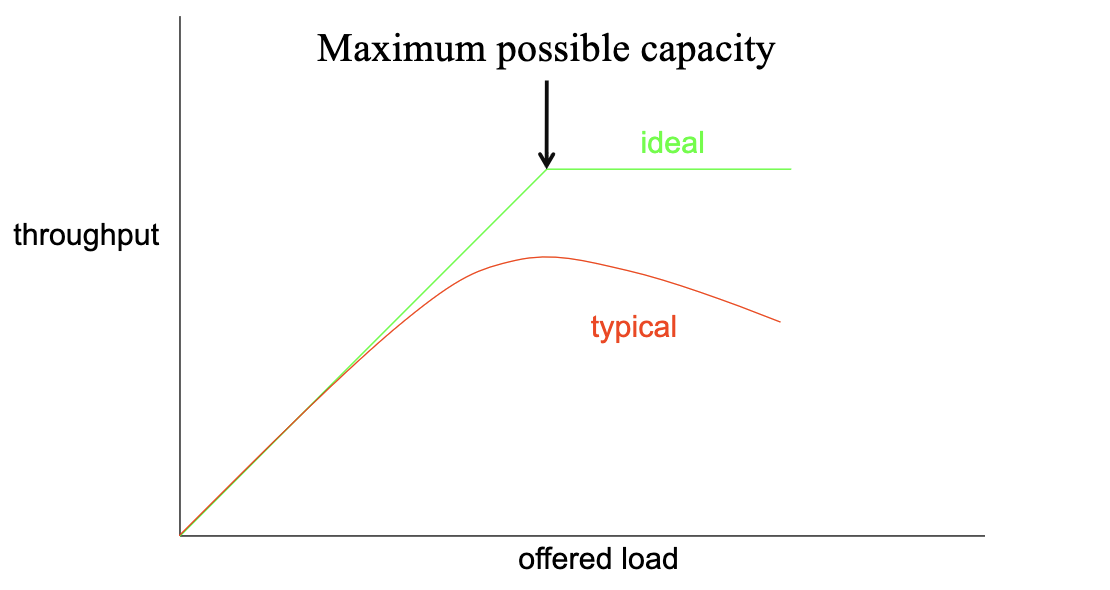
\includegraphics[scale=0.4]{images/throughput.png}
\end{center}

This happens because scheduling isn't free! It takes time to dispatch a process (overhead). More
dispatches mean more overhead (lost time). Consequently, less time (per second) is available to run
processes. Naturally, we can try minimizing the performance gap by reducing the overhead per dispatch and minimize the
number of dispatches.
\exampleEnd

\exampleBegin{Delay Doozy}
\begin{center}
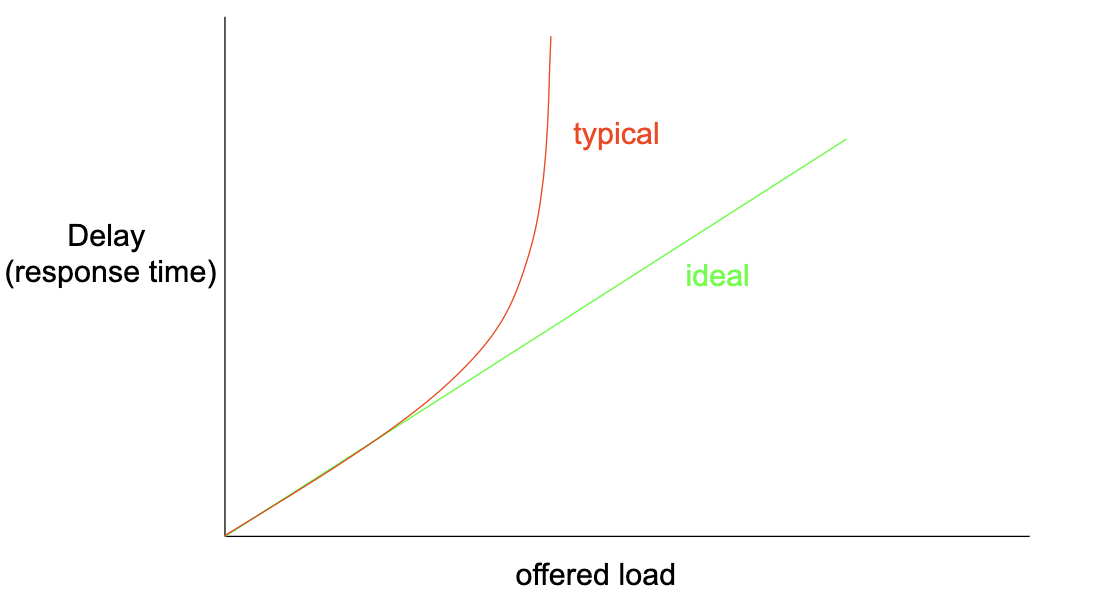
\includegraphics[scale=0.4]{images/delay.png}
\end{center}

This happens because real systems (unfortunately) have finite limits (like queue size). When limits
are exceeded, requests are typically \textit{dropped}\footnote{Dropped: We simply don't process the
  request}. From the requester's view, this looks like an infinite response time since the request
isn't begin serviced at all! Even if there are mechanisms like automatic retries (e.g. TCP
retransmissions), the retries themselves could also be dropped, further exacerbating the
situation. During these periods of heavy loads, the system performance drops severely since
overheads like context switching and memory management will explode. Careful system design and resource management can help to minimize this problem, but it is not
guaranteed to \textit{fix} the problem.
\exampleEnd

\subsubsection*{Graceful Degradation}
\addcontentsline{toc}{subsubsection}{Graceful Degradation}
\definitionBegin{Overload and Graceful Degradation}
A system is said to be \textbf{overloaded} when it can no longer meet its service goals.
\tcblower
\textbf{Graceful degradation} ensures that the system will continue service, but with degraded
performance.
\definitionEnd

When a system is overloaded, we want to use the graceful degradation principle to at least do
\textit{some} work. We \textit{never} want to allow throughput to drop to zero. This will allow
response times to grow without limit; i.e. this will lead to infinite response times!


\subsection{Non-Preemptive Algorithms}


\subsubsection{First Come First Serve}
The First Come First Serve (FCFS) algorithm consists of running the processes in the order that they
arrived. We run the first process on the ready queue until it completes or yields. One of the
primary characteristics of this algorithm is that it has highly variable delays since it relies on
the process order.

\bookBegin{FIFO/FCFS}
What happens when we relax assumption \textit{(i)} (See \textbf{\nameref{subsubsec:SM}})? Well,
long-running processes will monopolize CPU time, delaying the execution of shorter processes! This
results in poorer performance if a long-running process runs first.
\bookEnd

While FCFS ensures that all processes will eventually be served, it may not be the most efficient
since it can result in poor utilization of the CPU and inefficient response times. Long-running
processes will monopolize CPU time, delaying the execution of shorter processes.


\subsubsection{Shortest Job First}
The Shortest Job First (SJF) algorithm runs the processes in the order of their run-times. We run
the process with the shortest run-time on the ready queue until it completes or yields. One of the
primary characteristics of this algorithm is that it optimizes for throughput (good for batch
processing!).

\bookBegin{FIFO/FCFS}
What happens when we relax assumption \textit{(ii)} (See \textbf{\nameref{subsubsec:SM}})? Well, we
run into the same problem as FCFS if the long-running process arrives first! The long-running
process will monopolize CPU time, delaying the execution of the other processes! 
\bookEnd





\subsection{Real-Time Schedulers}
Real-time schedulers are used in systems with time-sensitive tasks. Deadlines can either be
\textit{hard}\footnote{Hard: Under no circumstances can the deadline be missed.} or
\textit{soft}\footnote{Soft: It isn't the end of the world if the deadline is missed.}.


\subsubsection{Hard}
Hard real-time schedulers rigorously enforce deadlines through careful analysis and pre-defined
schedules. Often times, this means that we know \textit{in advance} the schedule of processes to be
run. Therefore, there is no nondeterminism in your scheduler, and it is inherently non-preemptive.
These real-time schedulers are uncommon. 

\exampleBegin{Deadly Deadline}
Assume you have to write a scheduling algorithm to control a nuclear power plant. If you miss a
particular process deadline, your plant will probably blow up. So, you carefully analyze your
processes to come up with the \textit{perfect} schedule that will \textit{never} miss a
deadline. Since you know the processes in advance, there is no nondeterminism in your
schedule.
\exampleEnd


\subsubsection{Soft}
Soft real-time schedulers \textit{want} to meet deadlines, but it won't be the end of the world if
they don't. So, we want to optimize our scheduler to avoid missing deadlines. We can do so by giving
each process a priority level: the higher the priority, the sooner the deadline.

One possible algorithm is Earliest Deadline First (EDF), which will sort jobs based on deadlines,
minimizing total lateness.

If deadlines are missed, the system's response depends on its design and may involve dropping the
job, falling behind, or dropping future jobs to compensate.

\exampleBegin{Choppy Video}
When watching a video, the reason why it may be choppy at times is because the scheduler will drop
certain packets that missed their deadline! Thus, to the end user it appears choppy, probably
because their internet sucks (they might be using eduroam).
\exampleEnd





\subsection{Preemptive Algorithms}
\bookBegin{Preemptive Algorithms}
When we relax \textit{(iii)} (See \textbf{\nameref{subsubsec:SM}}), we get preemptive algorithms.
\bookEnd


\subsubsection*{Preface: Implementing Preemption}
\addcontentsline{toc}{subsubsection}{Implementing Preemption}
Preemption can be caused by syscalls or clock interrupts. Before returning control to the process,
the scheduler is consulted to determine if there are higher-priority ready processes or any
processes that need to be woken up. The scheduler will find the highest priority ready process,
switching to it (if it's not the current process), effectively preempting the current process.

We can use clock interrupts to do this. Modern CPU's have a clock peripheral device that can
generate interrupts at fixed time intervals. These clock interrupts will temporarily halt the
currently running process, transferring control to the scheduler, allowing for preemptive scheduling.


\subsubsection{Round Robin}
\label{subsubsec:RR}
The Round Robin (RR) algorithm consists of assigning a time slice to all processes (usually the same
size). Processes are scheduled as they arrive and run until they either block or their time slice
expires. After running, the process is put at the end of the process queue. Eventually each process
will get a turn to run for its allotted time slice.

Some key characteristics of RR is that this usually results in faster response times (for
interactive applications), but since more context switches occur, they can be
expensive. Additionally, runaway processes have less impact since they only take a fraction of the
overall cycles, and will not run forever.

\bookBegin{Round Robin}
Note that ``fair'' algorithms like RR will perform poorly in turnaround time. Thus, we use response
time to measure such algorithms. Now, relaxing assumption \textit{(iv)} (See
\textbf{\nameref{subsubsec:SM}}), we can see that there may be gaps where the CPU isn't doing
anything! To remedy this, we want to move the process to the back of the process queue whenever the
process halts, \textit{regardless} of how (I/O, interrupt, etc.). This way, the CPU is
\textit{always} doing something useful.
\bookEnd

\subsubsection{Choosing a Time Slice}
The duration of the time slice is crucial for optimizing performance. Longer time slices reduce the
frequency of context switches, but are bad for response times. Shorter time slices are better for
response time, but are more expensive since they require more context switches. Striking the right
balance is important!


\subsubsection{Cost of Context Switches}
When a context switch occurs, the OS goes through several steps, handling the interrupt, saving
register values, and invoking the scheduler, all of which incur overhead. Additionally, context
switching involves changing the stack and handling non-resident process descriptions. Furthermore,
the switch requires mapping out the old and new processes, affecting the efficiency of address space
changes. More notably, the loss of instruction and data caches significantly impacts the speed of
subsequent instructions, reducing overall performance.


\subsection{Priority Algorithms}
\definitionBegin{Starvation}
\textbf{Starvation} refers to when processes that have low priority don't run very often or don't
run at all.
\definitionEnd

Priority scheduling assigns each process a particular priority level (higher usually meaning more
important). Priority scheduling depends on if the scheduler is preemptive or
non-preemptive. Non-preemptive priority schedules simply dictate the order the processes will run
in. However, if the scheduler is preemptive, we may have a case where, when a new process is
created, it preempts the running process (assuming the new process has higher priority). One concern
for preemptive priority algorithms is the possibility of starvation.


\subsubsection{Hard and Soft}
\definitionBegin{Hard and Soft Priorities}
A \textbf{hard priority} refers to when processes with the highest priority has absolute precedence
over lower-priority processes and can preempt them to gain immediate access to the resource.
\tcblower
A \textbf{soft priority} refers to when resources are allocated according to their priority
level. Higher priority processes receive a larger share of resources, but lower-priority
processes aren't blocked entirely.
\definitionEnd

\exampleBegin{Linux Priorities}
Linux uses soft priorities, represented by a ``nice value'' assigned to each process. The nice value
indicates the share of CPU resources a process should receive. Users can adjust priorities using
specific commands, but can only request \textit{lower} priorities. Higher priorities can only be
requested by privileged users.
\exampleEnd


\subsubsection{Multi-Level Feedback Queue}
\bookBegin{Multi-Level Feedback Queue}
What happens when we relax assumption \textit{(iii)} (See \textbf{\nameref{subsubsec:SM}})? We get
the Multi-Level Feedback Queue! This scheduler is so important that there's an entire chapter
dedicated to it!
\bookEnd

The Multi-Level Feedback Queue (MLFQ) is a technique that uses multiple ready queues with varying
time slices to accommodate different types of processes. We want to optimize both response time for
interactive tasks and minimize overhead for longer background tasks. The foreground queue with
shorter time slices (high priority) is used for quick responses. The background queue with longer
time slices (low priority) minimizes overhead.

When a new process enters the scheduler, it is initially placed in the high priority queue. Once its
time slice expires, the process is then moved to the low priority queue. Periodically, all processes
are moved back to the high priority queue to prevent starvation!

MLFQ achieves acceptable response times for interactive jobs without wasting CPU
resources. Additionally, the scheduler dynamically adjusts based on the actual behavior of jobs,
providing an automatic and adaptive scheduler!





\section{Memory Management}
There are three primary goals for memory management:
\begin{enumerate}[label=\textit{(\roman*)}]
\item Transparency: Processes should only be able to see their own address space. That is, their
  address space is isolated, and processes are oblivious of any memory sharing with other
  processes. This ensures data privacy and security.
\item Efficiency: The system should utilize memory efficiently to optimize resource allocation and
  minimize waste. The allocation and (when necessary) relocation of memory should be performed with
  low run-time overhead to maximize system performance.
\item Protection and isolation: We want to ensure that the data within a process remains protected
  and is isolated from outside processes. That is, other processes can neither access it nor modify
  it.
\end{enumerate}
The memory management problem involves several key aspects:
\begin{enumerate}[label=\textit{(\roman*)}]
\item Unpredictability: Processes usually cannot accurately predict the exact amount of memory they
  will require during execution.
\item Continuity Expectations: Processes expect to find their existing data where they left it,
  implying that processes assume they have a contiguous address space.
\item Limited Physical Memory: The total memory required by all the processes may exceed the
  available physical memory.
\item Efficient Process Switching: We need to optimize the delay for copying data.
\item Low Overhead: The cost of memory management should be minimized to maximize system performance.
\end{enumerate}


\subsection*{Preface: Physical and Virtual Addresses}
\addcontentsline{toc}{subsection}{Preface: Physical and Virtual Addresses}
\definitionBegin{Physical and Virtual Memory Addresses}
\textbf{Physical memory addresses} refer to the actual hardware location of a particular memory
block.
\tcblower
\textbf{Virtual memory addresses} are an \textit{abstraction} over physical memory addresses, and
are \textit{not} the same as physical addresses. They represent a contiguous block of memory, when
in reality the physical addresses may be scattered.
\definitionEnd

Virtual memory addresses are used in processes and allow for more flexibility in memory management,
but require a virtual to physical translation unit. 


\subsection*{Preface: Fragmentation}
\addcontentsline{toc}{subsection}{Preface: Fragmentation}

\definitionBegin{Internal and External Fragmentation}
\textbf{Internal fragmentation} occurs when there is wasted space \textit{inside} a block of
allocated memory. That is, the requester was given more memory than he needed.
\tcblower
\textbf{External fragmentation} occurs when there is free space in the memory that cannot be used to
satisfy any memory allocation request since the available free memory is fragmented into smaller,
non-contiguous blocks. As a result, the total amount of free memory may satisfy the request, but
since the memory isn't contiguous, we cannot fulfill it.
\definitionEnd

\subsection{Fixed Partition Allocation}
Fixed Partition Allocation divides the available memory into fixed-size partitions (go figure), and
each partition is assigned to a specific process. The number of partitions is pre-allocated and is
based off the expected number of processes and their sizes. Each process can only access the
partition assigned to it and cannot access the memory allocated to other processes.

This approach is relatively easy to implement and was used in early batch processing systems. The
de/allocation of partitions are straightforward and efficient. However, it is not very flexible
since it requires a predetermined number of partitions and may lead to inefficient memory
utilization if the partition sizes are not well-matched with the actual memory requirements of the
processes.

To enforce memory protection, hardware support is often used. Special registers that hold the
partition boundaries ensure that each process can only access memory within its allocated
partition. However, fixed partition allocation does not use virtual addresses, meaning the processes
use the physical addresses directly.

\subsubsection{Problems}
There are several problems with Fixed Partition Allocation:
\begin{enumerate}[label=\textit{(\roman*)}]
\item Static Allocation: Fixed Partition Allocation requires knowing the exact memory requirements
  of all processes in advance, making it challenging to handle dynamic memory demands.
\item Limitations: The number of partitions defines the maximum number of processes that can be
  accommodated concurrently. If the partitions are not efficiently sized or the number of processes
  exceed the partition count, some processes may not be able to run concurrently.
\item Inefficient: Some partitions may be unused or underutilized, leading to poor memory
  utilization.
\item Limited Sharing: Processes cannot easily share memory, making it difficult to implement
  communication and data sharing between processes.
\item Internal Fragmentation: If partitions are not efficiently sized, they may succumb to internal
  fragmentation, leading to wasted memory.
\end{enumerate}
Because of these reasons, this approach isn't commonly used in modern operating systems.


\subsection{Dynamic Partition Allocation}
Dynamic Partition Allocation allows variable-sized partitions which accommodate almost any size
requested. Each partition has contiguous addresses, and processes are allowed to access the
partitions it requested. These partitions can be shared between multiple processes, and a single
process may have multiple partitions with different sizes and characteristics. However, in the basic
scheme, memory addresses are still physical, which can lead to external fragmentation and limited
address space. 

\subsubsection{Problems}
There are several problems with Dynamic Partition Allocation:
\begin{enumerate}[label=\textit{(\roman*)}]
\item Not Relocatable: Once a partition is allocated, it is very hard to relocate its contents to
  another memory location, which can lead to inefficient memory utilization.
\item Not Expandable: Dynamic partitions are limited in their ability to grow/shrink to
  accommodate changing memory requirements of processes.
\item Limited Support: Dynamic partitions may struggle to support address spaces larger than
  physical memory, hindering their ability to handle memory-intensive jobs.
\item External Fragmentation: As processes de/allocate memory over time, dynamic partitions can
  suffer from external fragmentation, leading to wasted memory.
\end{enumerate}
Relocation and expansion can be challenging in dynamic partition allocation because partitions
are tied to specific address ranges during execution. Relocating the contents of a partition require
updating all the pointers within the contents, which is not always feasible, especially if you don't
know which memory locations contain pointers. Additionally, expanding a partition may be challenging
since there may not be enough contiguous free space. These limit the usefulness of dynamic partition
allocation. 


\subsection*{Managing Variable-Sized Partitions}
\definitionBegin{Free List}
The \textbf{free list} is a data structure (often implmented with a list or array) that keeps track
of all available chunks of unallocated memory.
\definitionEnd

To manage variable-sized partitions, the memory manager starts with a single large block of memory
known as the ``heap'', and maintains a data structure called the ``free list''. When a process
requests memory, the memory manager will consult the free list, carving a chunk (of the requested
size) and putting the remainder back onto the free list. When processes deallocate memory, it is put
back onto the free list.


\subsection{Free-Space Management}
Fixed sized blocks are easy to track: we can use a bitmap to indicate which blocks are free.

Variable chunks require more information. Each chunk of memory has a descriptor containing
information about its free status, chunk size, and a pointer to the next chunk. These chunks are
typically organized into a linked list.

Variable sized partitions are not as subject to internal fragmentation since processes, in theory,
request the exact amount of memory needed. However, they are subject to external fragmentation. We
can minimize external fragmentation by consulting an algorithm to determine how we manage our free
list.


\subsubsection{Best Fit}
The best fit algorithm will search for the \textit{smallest} available chunk that meets the size
requirements. This minimizes memory waste and reduces internal fragmentation.

\begin{tcbraster}[raster columns=2, raster equal height, raster force size=false]
  \begin{tcolorbox}[colback=green!5!white,colframe=black!75!green,title=Advantages]
    \begin{enumerate}[label=\textit{(\roman*)}]
    \item Increased odds of a (near) perfect fit.
    \end{enumerate}
  \end{tcolorbox}
  \begin{tcolorbox}[colback=red!5!white,colframe=black!40!red,title=Disadvantages]
    \begin{enumerate}[label=\textit{(\roman*)}]
    \item An exhaustive search is necessary.
    \item Quickly creates small fragments.
    \end{enumerate}
  \end{tcolorbox}
\end{tcbraster}


\subsubsection{Worst Fit}
The worst fit algorithm will search for the \textit{largest} available chunk that meets the size
requirements. This tries to minimize memory waste by creating large fragments.

\begin{tcbraster}[raster columns=2, raster equal height, raster force size=false]
  \begin{tcolorbox}[colback=green!5!white,colframe=black!75!green,title=Advantages]
    \begin{enumerate}[label=\textit{(\roman*)}]
    \item Tends to create large fragments.
    \end{enumerate}
  \end{tcolorbox}
  \begin{tcolorbox}[colback=red!5!white,colframe=black!40!red,title=Disadvantages]
    \begin{enumerate}[label=\textit{(\roman*)}]
    \item An exhaustive search is necessary.
    \item Over time, small fragments are inevitable.
    \end{enumerate}
  \end{tcolorbox}
\end{tcbraster}


\subsubsection{First Fit}
The first fit algorithm will search for the \textit{first} available chunk that meets the size
requirements. This reduces overhead since there's no need (potentially) to search exhaustively.

\begin{tcbraster}[raster columns=2, raster equal height, raster force size=false]
  \begin{tcolorbox}[colback=green!5!white,colframe=black!75!green,title=Advantages]
    \begin{enumerate}[label=\textit{(\roman*)}]
    \item Creates random sized fragments.
    \item Doesn't require an exhaustive search.
    \end{enumerate}
  \end{tcolorbox}
  \begin{tcolorbox}[colback=red!5!white,colframe=black!40!red,title=Disadvantages]
    \begin{enumerate}[label=\textit{(\roman*)}]
    \item The first chunks quickly fragment
    \item Over time, the searches become longer.
    \end{enumerate}
  \end{tcolorbox}
\end{tcbraster}


\subsubsection{Next Fit}
The next fit algorithm will search for the \textit{first} available chunk that meets the size
requirements \textit{starting from the last allocation point} instead of the beginning of the free
list. This reduces overhead and tries to minimize fragmentation.

\begin{tcbraster}[raster columns=2, raster equal height, raster force size=false]
  \begin{tcolorbox}[colback=green!5!white,colframe=black!75!green,title=Advantages]
    \begin{enumerate}[label=\textit{(\roman*)}]
    \item Creates random sized fragments.
    \item Reduces overhead since we don't start from the beginning.
    \end{enumerate}
  \end{tcolorbox}
  \begin{tcolorbox}[colback=red!5!white,colframe=black!40!red,title=Disadvantages]
    \begin{enumerate}[label=\textit{(\roman*)}]
    \item Over time, memory chunks still fragment.
    \item Over time, the searches become longer.
    \end{enumerate}
  \end{tcolorbox}
\end{tcbraster}


\subsection{Coalescing Partitions}
Coalescing partitions is a technique used to reduce external fragmentation in variable-sized
partition allocation algorithms. When a process frees a chunk of memory, the memory management
system checks if the neighboring chunks are also free. If they are, the system combines them into a
larger, contiguous block, reducing fragmentation.

\bookBegin{Free-Space Management}
To simplify the coalescing process, we can organize the free list such that neighboring chunks are
placed close to each other. One way to do this is by ordering the free list by addresses, making it
more efficient to find neighboring chunks and merge them when necessary.
\bookEnd

Coalescing helps minimize external fragmentation by reducing the number of small, unusable gaps
between allocated memory blocks. However, it is worth noting that it doesn't \textit{completely}
eliminate external fragmentation since it can only merge \textit{contiguous} chunks.

When multiple processes operate in parallel, it's challenging to predict which process will dominate
and how they will interact, leading to potential fragmentation issues. The fraction of space
typically allocated depends on the number and size of processes running; if a significant portion of
memory is allocated, coalescing becomes less effective due to limited free space.

Additionally, the speed of allocated memory turnover affects coalescing; processes holding memory
chunks for extended periods reduce the effectiveness of coalescing. Note that coalescing only
minimizes fragmentation since external fragmentation will \textit{always} occur over time.


\subsection{Buffer Pools}
Certain chunk sizes are requested more frequently than others. Key services like I/O, network
protocols, etc. usually work with fixed-size buffers. Thus, we can reserve special pools of
fixed-size buffers for popular buffer sizes.

\definitionBegin{Buffer Pool}
A \textbf{buffer pool} is a reserved section of fixed-sized memory buffers used to handle frequently
requested memory sizes (like Reiher's favorite 4K), reducing memory management overhead and external
fragmentation.
\definitionEnd

Buffer pools are used to handle frequently requested memory sizes efficiently. When there are
popular buffer sizes, the operating system can reserve special pools of fixed-size
buffers. When a request for a matching buffer size arrives, it is taken out of the buffer pool as
opposed to the free list. This reduces external fragmentation and memory management overhead.

However, the OS needs to determine an appropriate size for the buffer pool. Too small and it might
not improve efficiency. Too large and it might lead to a lot of unused buffer space.
It is also worth noting that buffer pools will only satisfy \textit{perfectly} matching requests,
since otherwise we get internal fragmentation.

\subsubsection{Sizing}
We dynamically adjust the size of the buffer pool based on the system load and buffer
availability. When the pool runs low on fixed-size buffers, we simply acquire more memory from the
free list\footnote{If the free list gets dangerously low, we ask each major service with a buffer
  pool to return space.} and divide it into new buffers. When the pool is too large, we release some
buffers back into the free list. We can tune these thresholds (low space and high space) to
determine when to adjust the buffer pool size. This approach makes the system highly adaptive to
changing workloads and memory requirements.

\subsection{Memory Leaks}
\definitionBegin{Memory Leak}
A \textbf{memory leak} is when memory is allocated but never freed, causing the memory to remain
occupied indefinitely.
\definitionEnd

Memory leaks in the context of buffer pools occur when a process is done with a buffer, but fails to
free it. This causes the buffer to remain in the pool indefinitely, wasting memory. Long running
processes with memory leaks can result in substantial memory waste over time. Addressing memory
leaks is crucial if we want efficient memory utilization.

\exampleBegin{Leaky Program}
Assume you have a small program that allocates some memory and immediately terminates. You are
surprised that there are no memory leaks! However, this is just because when a process dies,
\textit{all} of its memory gets reclaimed, \textit{implicitly} freeing the memory you allocated in
your program. But what if you had a \texttt{while (true)} loop in your code? Since you aren't doing
anything with that memory, it's probably a good idea to let someone else use it! But, since you
never explicitly freed it, the memory you allocated is inaccessible (until the process terminates)!
Because of this, It is generally bad practice to not \textit{explicitly} free any memory you
\textit{explicitly} allocate. 
\exampleEnd


\subsection{Garbage Collection}
Garbage collection (GC) is a technique to address memory leaks and reclaim unused memory. Instead of
relying on processes to release memory on their own, garbage collection monitors the amount of free
memory left on the system. When there is \textit{memory pressure}\footnote{Memory pressure: When the
  amount of free memory becomes dangerously low.}, garbage collection is triggered.

The system will search the data space to identify all reachable objects, noting their address and
size. Then, any unreachable objects (inaccessible memory) is then reclaimed and added back into the
free list. This ensures that memory is efficiently utilized and helps prevent memory leaks!


\subsubsection{Determining Accessible Memory}
In general, we want to identify and reclaim memory that is no longer used. To do this, we do the
following:

\begin{enumerate}[label=\textit{(\roman*)}]
\item Find all pointers in allocated memory: We need to traverse \textit{all} allocated memory to
  locate the pointers that reference other objects/data.
\item Determine the size of each pointer: We must determine the size and extent of the memory
  region each pointer references.
\item Determine what is/n't pointed to: We need to identify objects that are still accessible and in
  use by actively referenced pointers.
\item Free inaccessible memory: We put all inaccessible memory back into the free list.
\end{enumerate}
GC can be difficult because it requires comprehensive scanning of the entire memory space to
identify references and determine object boundaries. Furthermore, it also needs to be able to handle
complex references (e.g. cyclic data structures) for accurate identification of unused
memory. Additionally, GC takes time, and therefore can slow down system performance.


\subsubsection{Problems}
There are several problems we need to address:
\begin{enumerate}[label=\textit{(\roman*)}]
\item Identifying pointers are \textit{hard}. Locations in a program's data or stack segments may
  \textit{appear} to contain addresses but are actually just data (that \textit{resembles}
  addresses). We need to accurately identify valid pointers to avoid reclaiming active memory.
\item Even if pointers are identified, we need to determine if they are still accessible and in use! This
  requires recursive analysis of dynamically allocated data structures to ensure that all referenced
  memory remains reachable. Even so, statically allocated data structures are harder to analyze.
\item We also need to determine the size of each object pointed to, which can be challenging! Measuring
  exact boundaries may be hard for complex data structures or objects with variables sizes.
\end{enumerate}


\subsection{Memory Compaction and Relocation}
GC is simply another method to release memory, and therefore doesn't significantly impact
fragmentation. Ongoing memory de/allocations can prevent coalescing, leading to fragmentation over
time\footnote{Frequent allocations can starve coalescing, reducing its effectiveness.}. 

To counter this, we can compact active memory to one end, coalescing the other end to eliminate
fragmentation! However, this requires relocation, which is extremely complicated, since we need to
update all memory references correctly.

When a process is relocated, all addresses within the program will become invalid, resulting in
potential errors and crashes. We would need to:

\begin{enumerate}[label=\textit{(\roman*)}]
\item Update all references in the code segment (e.g. calls and branches to other parts of code) to
  point to the correct memory addresses in the new location.
\item Update referees to variables in the data segment to point to the correct addresses in the new
  location.
\item Ensure that new pointers are adjusted to point to the correct addresses after relocation.
\end{enumerate}
To solve the relocation problem, we can make the process location independent! By doing this, we can
avoid the complexities of update memory references, \textit{abstracting} away \textit{(i) -- (iii)}! We want to enable processes to execute in \textit{any} part of memory
without adjusting memory addresses. 

We can achieve this using various techniques:
\begin{enumerate}[label=\textit{(\roman*)}]
\item Relative addressing: We can use offsets instead of absolute memory addresses to allow
  processes to be loaded into different memory locations with no address modifications.
\item Base and Bounds Registers: We can use hardware registers (base and bound registers) to
  automatically adjust memory references at runtime. These registers keep track of the base address
  and size (bound) of the process' memory space, allowing the CPU to translate relative addresses
  into absolute addresses during execution.
\item Virtual Memory and Paging: We can use VM techniques like paging to abstract the physical
  memory from the process' address space. This way, the process can work with the virtual addresses
  that get translated to physical addresses, making the process independent of its location.
\end{enumerate}

\abstractionBegin{Virtual Memory}
Virtual memory is an \textit{abstraction} over physical memory! A virtual address is \textit{not}
the same as its corresponding physical address, and requires a translation unit to convert between
the two. However, this is a small price to pay for making memory relocation \textit{significantly}
easier!
\abstractionEnd

\subsubsection{Segment Relocation}
Memory segment relocation is a technique that involves organizing a process' address space into
multiple segments, each representing a contiguous block of memory with a specific purpose (see
\refto{subsec}{PAS}). The segments are then moved as a unit during relocation.


\subsubsection{Base and Bounds Registers}
Computer architecture may include special relocation registers known as segment \textit{base
registers}. These registers hold the starting address of each segment in physical memory. When the
CPU accesses a memory location, it will add the address to the address of the base register,
translating the virtual address to the physical address!

When a program is loaded into memory, the OS sets the base registers to the start of the
program. When relocating, we simply update the base register accordingly. This way, the program can
continue to run smoothly regardless of where it is located in physical memory.


\subsubsection*{Corollary: Security}
\addcontentsline{toc}{subsubsection}{Corollary: Security}
We still need to protect our memory! Protection refers to preventing a process from accessing memory
outside its allocated memory. To achieve this, we utilize a length (or limit) register, often
called the \textit{bounds register}, which specifies the maximum valid offset from the start of the
segment. Any address greater than the limit is considered illegal and should be inaccessible to the
process. 

When processes attempt to access an illegal address, the CPU triggers a segmentation exception or
trap. This exception traps into the OS allowing it to take appropriate action (e.g. terminating the
process or controlling the violation).


\subsection{Swapping}
Swapping is a technique to overcome the limitation of physical RAM by temporarily storing inactive
processes' memory on disk. When a process isn't actively running (e.g. yields, blocked), its entire
memory contents are copied to disk to free up RAM for other processes.

When a process is scheduled to run again, its memory is then copied back from disk onto RAM to
continue execution. If the system has relocation hardware, the memory can be placed in different RAM
locations, enabling processes to access their memory regardless of their physical addresses. This
allows the system to use disk space as a virtual extension of physical memory, giving the 
\textit{illusion} that each process gets all of RAM to itself. 

However, swapping incurs overhead since copying is expensive! The cost of a context switch are
\textit{very} high, since we need to:

\begin{enumerate}[label=\textit{(\roman*)}]
\item Copy all of RAM out to disk.
\item Copy other stuff from disk to RAM.
\end{enumerate}
\textit{before} the new process can do anything. Moreover, we still cannot exceed the amount of
physical RAM, which can limit memory-intensive processes or overall system performance.


\subsection{Paging}
Paging is a technique that divides both physical memory and virtual address space into fixed-size
units\footnote{Usually 1-4K bytes or words.} called \textit{pages}. The pages in physical memory are
referred to as \textit{page frames}, while pages in virtual memory are just called \textit{pages}.

Each virtual page is mapped to a physical page frame, but it's not fixed nor is it
one-to-one. Instead, a per-page translation mechanism called a \textit{memory management unit
  (MMU)}\footnote{The Memory Management Unit (MMU) is hardware (often integrated into the CPU)
  responsible for handling memory access and virtual-to-physical address translation.},
is used to dynamically translate virtual page numbers to corresponding physical page frame
numbers. 


\subsubsection{Big Page Tables}
\definitionBegin{Translation Lookaside Buffer}
The \textbf{Translation Lookaside Buffer (TLB)} is the MMU cache that stores a subset of recently
accessed page table entries. This improves lookup times since we don't have to access page table
entries from main memory for \textit{every} memory access.
\definitionEnd

Traditionally, page tables were implementing using fast registers in the MMU. But with larger memory
sizes and smaller page sizes, there will be a \textit{lot} of pages.

\exampleBegin{How Many Pages?}
Suppose you have 64 GB memory with 4K page sizes. There would be $\frac{64 \textit{GB}}{16
  \textit{KB}} = 16$ \textit{million} pages! Unfortunately, we cannot afford to store 16 million
pages into fast registers. 
\exampleEnd

\definitionBegin{TLB Hit and Miss}
A \textbf{TLB hit} is when the required translation is found in the TLB.
\tcblower
A \textbf{TLB miss} is when the required translation is \textit{not} in the TLB, and an access to
the page table is necessary.
\definitionEnd
To remedy this, TLB's act as a high-speed cache for virtual-to-physical address translations,
reducing overhead. When the CPU needs to translate a virtual address, it first checks the TLB. If
the translation is found in the TLB, we return it. Otherwise, we need to consult the page table in
main memory to retrieve the required page table entry. The TLB is then updated accordingly.

Unfortunately, the TLB has a limited size, and therefore not all entries can fit into it. This lead
to the issue of cache invalidation and replacing entries when the TLB is full. Maintaining a high
TLB hit ratio is crucial for efficient VM performance.


\subsubsection{Swap Space}
\definitionBegin{Page Fault}
A \textbf{page fault} is when the required address is not in the TLB, is valid, but is not present
(i.e. it is in the swap space or page file). 
\definitionEnd

Since we have more pages than RAM, we need to store some of them somewhere other than
RAM. Typically, some pages are kept on disk and are referred to as the \textit{swap space} or
\textit{page file}. When a page fault occurs, the OS retrieves\footnote{In the meantime, other
  processes can execute} the required page from the swap space, loading it into an available page
frame in RAM. The program counter is backed up to retry the failed instruction after the page is
loaded, allowing the process to continue running.  


\subsubsection{Ongoing Operations}
The MMU has many ongoing operations. Here are three important ones:
\begin{enumerate}[label=\textit{(\roman*)}]
\item Adding/Removing Pages: When the current process dynamically de/allocates memory, the MMU
  needs to reflect this in the page table. The OS will directly update the active page table in
  memory to adjust the relevant page mappings. A privileged instruction is used to flush any stale
  cached entries in the MMU to ensure an accurate mapping.
\item Context Switching: When the system switches processes, the MMU needs to switch the appropriate
  page table for the new process. Each process has a separate page table, and a privileged
  instruction is used to load the pointer to the new page table. Before the new process begins
  execution, a reload instruction flushes any previously cached entries, preventing invalid access.
\item Page Sharing: Page sharing allows for memory sharing between multiple processes. The page
  tables can be configured to point to the same \textit{physical} page. This means multiple
  processes can have access to the same page in RAM. Page sharing can be read/write or read-only
  depending on access requirements and memory protection mechanisms enforced by the OS. This
  approach is good for sharing read-only data (e.g. code segments, shared libraries), reducing
  redundancy.
\end{enumerate}


\subsubsection{Demand Paging}
Demand paging is a technique where not all pages of a process are loaded into RAM at once. Rather,
only pages that are actively being referenced are brought into memory when needed, allowing for
better memory efficiency and less overhead during process scheduling and context switching.

Demand paging frees up RAM by keeping the majority of a process' data on disk until it's actually
needed, enabling the system to accommodate more processes and improves overall memory
utilization. Demand paging utilizes page faults to signal when pages need to be fetched from disk. 

One problem of demand paging is performance optimization. Frequent page faults incur overhead since
the time it takes to fetch from disk can add up. Efficient page replacement algorithms like
\textit{Least Recently Used (LRU)}\footnote{The page that hasn't been accessed for the longest
  period of time is booted from RAM.} are used to minimize the number of page faults triggered to
ensure that relevant pages are kept in RAM.

\subsubsection{Locality of Reference}
Locality of reference suggests that the next address a program will access is most likely to be
close to the one it just accessed. This is usually present in programs since they often execute
sequences of consecutive (or nearby) instructions, have short branches, access data in the
current/previous stack frame, and (tend to) access recently allocated heap structures. While there
are no guarantees, identifying these trends help reduce the number of page faults.





\section{Virtual Memory}
Virtual memory (VM) is a generalization of demand paging, and is a technique that provides a large
and uniform address space to each process. It gives the \textit{illusion} that each process has
access to a vast amount of memory (much larger than the physical RAM available).

\abstractionBegin{Virtual Memory and Paging}
Virtual memory is an \textit{abstraction} over demand paging. It extends the concept of paging by
providing a much larger address space to each process by using dynamic paging and swapping.
\abstractionEnd

Processes can directly request segments in this space, and the virtual memory system handles the
mapping of virtual to physical addresses via page tables. VM allows processes to run even if their
entire address space doesn't fit into physical memory. Instead, only actively referenced portions
are loaded into RAM, while the rest sits on disk.

\subsection{Replacement Algorithms}
Replacement algorithms are the key technology to making virtual memory work. We want to have the
relevant pages loaded into RAM when a process needs to access them.

We do this by relying on the principle of locality of reference. Doing this allows us to make smart
choices about which pages to keep in memory and which ones to kick to disk.

Page replacement happens when we need to free up space in memory for new pages. Whenever a page
fault occurs, we select an appropriate page to replace via an algorithm (like LRU).

\subsubsection{The Optimal Algorithm (Belady's Algorithm)}
The optimal replacement algorithm replaces the page that will be accessed furthest into the future,
minimizing the number of page faults. However, this requires an oracle, and as such, it is
impossible to implement. This algorithm is also known as ``Belady's Algorithm''.


\subsubsection{FIFO and Random}
According to Reiher (and common sense), these are dogshit so I'm not going to cover them.

\subsubsection{Least Frequently Used}
The Least Frequently Used (LFU) policy kicks the least frequently used page back to disk. It isn't
the best in the world.

\subsubsection{Least Recently Used and Clock Algorithm}
Least Recently Used (LRU) policy kicks the page with the oldest timestamp back to disk. This is done
(naïvely) by timestamping each time a page is accessed. When a page needs to be replaced, we search
through all pages to kick the one with the oldest timestamp. This incurs a lot of overhead and
therefore is not commonly used.

Rather, we usually use an approximate LRU, or ``Clock Algorithm''. We maintain a circular buffer of
pages in memory, with each page having an additional reference/use bit (typically stored in the
MMU). When a page is accessed, we set the reference bit to 1, indicating it has been recently
used. When determining the page to replace, we scan starting at a fixed point, replacing the first
page with reference bit 0.

This algorithm, while not a perfect one-to-one with LRU, offers performance on par with LRU for a
fraction of the cost. Therefore, it is usually implemented in favor of a ``true'' LRU.


\subsection{Page Replacement}
We don't want to clear out \textit{all} page frames on each context switch as it can be
inefficient. There are several ways to deal with this:

\begin{enumerate}[label=\textit{(\roman*)}]
\item Single Global Pool: All processes share a single pool of page frames in memory. When a process
  runs, it uses any available free page frame for its page.
\item Fixed Allocation per Process: Each process is assigned a fixed number of page frames when it
  starts. The number of page frames stays constant throughout execution.
\item Working Set-Based Allocations: The working set of a process represents the set of pages it is
  actively referencing at any given time. Page frames are allocated dynamically based on a process'
  working set. When a process runs, its working set is loaded into RAM, and when it's switch out,
  its page frames are potentially freed.
\end{enumerate}


\subsubsection{Single Global Pool}
In the Single Global Pool approach, all page frames in memory are treated as a shared resource, and
an approximation of LRU is used as the replacement algorithm. However, this sucks when paired with
round-robin scheduling (see \refto{subsubsec}{RR}).

\exampleBegin{Fair or Unfair}
In RR scheduling, the process that was last in the queue will find all of its pages swapped
out. Thus, when this process runs, it will experience a high volume of page faults since all of its
pages were replaced.
\exampleEnd

This is because this approach doesn't account for the specific working sets of each process. For
this reason, this approach is usually pretty dogshit.


\subsubsection{Per-Process Pools}
In the Per-Process Pool approach, a fixed number of pages are allocated for each process, and the
approximate LRU is used \textit{separately} for each process. This allows for dynamic and customized
allocation of page frames to each process.

However, a fixed number of pages per process sucks because different processes exhibit varying
levels of locality, and the pages needed by each process usually change over time. Moreover,
processes have different natural scheduling intervals, and as such, their memory requirements vary
throughout execution!


\subsubsection{Working Sets}
\definitionBegin{Working Set}
A \textbf{working set} is defined to be the set of pages a process actively referenced within a
fixed sampling interval in the immediate past.
\definitionEnd

Working sets are used to allocate page frames to each running process based on its specific memory
needs. We allocate a sufficient number of page frames to hold each process' working set. This
ensures that the frequency of accessed pages are kept in memory, reducing the volume of page
faults. Each process will manage its own set of pages, usually using an approximate LRU for page
replacement. 

Working sets dynamically adjust the allocation of page frames for each process based on its current
behavior, optimizing memory usage and responding to changes in workload and access patterns.

\subsubsection*{Optimal Working Sets}
The optimal working set for a process is the set of pages it needs during its next time slice (or a
specific period of time). Allocating less than the optimal amount leads to a lot of page faults.

We determine the size of the working set by observing the process' behavior over time. Tracking the
frequency of page faults and memory references, the system can identify which pages the process
frequently accesses, including them in the working set.

\subsubsection*{Page Stealing: Working Set-Clock Algorithm}
The Working Set-Clock algorithm tracks the last use time for each page for its owning process,
replacing the page that was least recently used.


\subsection{Thrashing}
\definitionBegin{Thrashing}
\textbf{Thrashing} refers to when a system spends a significant amount of time/resources swapping
pages between RAM and disk, but isn't able to efficiently make any progress in the executing
process.
\definitionEnd

Thrashing occurs when the total demand for memory by \textit{all} running processes exceeds the
available physical memory. When thrashing happens, we seldom execute any useful instructions since
so much time is spent swapping pages. This results in an underutilized CPU and degraded performance.

Thrashing typically happens hen the working set of each process exceeds the available physical
memory. When there are not enough page frames to accommodate the working sets of all active
processes, they constantly compete for memory.

To protect against thrashing, the OS takes proactive measures like reducing the degree of
multiprogramming (i.e. limiting the number of active processes), using page replacement algorithms
that prioritize larger working sets, or allocating more physical memory (lol). The goal is to avoid
thrashing by ensuring that each process has enough pages in memory to execute efficiently.

\exampleBegin{Everyone Gets a Turn}
When reducing multiprogramming, we can use a RR approach for swapping processes in and out of disk,
ensuring that all processes get a fair share of CPU time while minimizing thrashing!
\exampleEnd


\subsection{Clean and Dirty Pages}
\definitionBegin{Clean and Dirty Pages}
A \textbf{clean page} refers to a page in memory that hasn't been modified since it was brought from
disk. They can be safely replaced without needed to write them back to disk since their contents
match that of the one on disk.
\tcblower
A \textbf{dirty page} refers to a page in memory that has been modified or updated after it was
brought from disk. That is, the in-memory version of the page is different from the one on disk. If
a dirty page needs to be removed from memory, the page must be written back to disk to update the
appropriate page on disk, ensuring that the most recent version of the data is saved before kicking
it from memory. 
\definitionEnd

When given a choice, the OS will prioritize kicking clean pages since they can be safely removed
without the need for I/O. Dirty pages however, need to be written back to disk to preserve data integrity.

\subsection{Preemptive Page Laundering}
Preemptive page laundering is a technique used to increase the flexibility of the memory manager by
converting dirty pages to clean ones. Rather than waiting to write when pages gets kicked, we
initiate a background write-out of dirty pages that are not actively in use. This way, we reduce
the risk of thrashing and increase the number of clean pages we have.





\section{Threads}
\definitionBegin{Thread}
A \textbf{thread} is a unit of execution and scheduling in a program. Each thread has its own stack,
program counter, and registers, allowing it to operate independently of other threads.
\definitionEnd

Threads within the same process share the same code and data segment, making them more efficient and
less resource-intensive than processes.

In multi-threaded programs, multiple threads can run concurrently within the same process. They
share the process' resources (e.g. memory, files), but each thread maintains its own execution
state. This allows for better communication and coordination between different parts of the
program.

They can be implemented and managed in various ways. User-level threads are managed by the process
itself and rely on voluntary yielding. Scheduled system threads are managed by the OS and can be
preemptively scheduled, meaning the OS can interrupt it to give other threads CPU time.


\subsection{Why Not Processes?}
Processes are expensive! Since each one has private resources and a private address space, it makes
interprocess communication difficult. Additionally, certain programs may not require such strong
separation. So, we can use threads to remedy such limitations of processes.

\subsection{Process v. Thread}
When should you use a process? A thread?

\begin{tcbraster}[raster columns=2, raster equal height, raster force size=false]
  \begin{tcolorbox}[colback=teal!5!white,colframe=black!75!teal,title=Processes]
    \begin{enumerate}[label=\textit{(\roman*)}]
    \item Running multiple, \textit{distinct} programs.
    \item Creation/destruction are \textit{rare} events.
    \item Running with distinct privileges.
    \item Limited interactions/shared resources.
    \item Strong separation between other processes.
    \end{enumerate}
  \end{tcolorbox}
  \begin{tcolorbox}[colback=yellow!5!white,colframe=black!75!yellow,title=Threads]
    \begin{enumerate}[label=\textit{(\roman*)}]
    \item Parallel activities in a \textit{single} program.
    \item Creation/destruction are \textit{frequent}.
    \item All can run with the same privilege.
    \item Need to shared resources.
    \item Frequent message/signal exchange.
    \item When you don't need protection from each other.
    \end{enumerate}
  \end{tcolorbox}
\end{tcbraster}


\subsubsection{Tradeoffs}

\subsubsection*{Processes}
\begin{tcbraster}[raster columns=2, raster equal height, raster force size=false]
  \begin{tcolorbox}[colback=green!5!white,colframe=black!75!green,title=Advantages]
    \begin{enumerate}[label=\textit{(\roman*)}]
    \item String isolation: Processes have distinct address spaces.
    \item Fault tolerance: Processes don't affect other processes.
    \item Easier resource cleanup: When a process terminates, all resources are automatically freed.
    \end{enumerate}
  \end{tcolorbox}
  \begin{tcolorbox}[colback=red!5!white,colframe=black!40!red,title=Disadvantages]
    \begin{enumerate}[label=\textit{(\roman*)}]
    \item Slower communication: Interprocess communication is more complex and slower.
    \item Potential duplication: Since each process has a distinct address space, this allows for
      unnecessary duplication.
    \end{enumerate}
  \end{tcolorbox}
\end{tcbraster}


\subsubsection*{Threads}
\begin{tcbraster}[raster columns=2, raster equal height, raster force size=false]
  \begin{tcolorbox}[colback=green!5!white,colframe=black!75!green,title=Advantages]
    \begin{enumerate}[label=\textit{(\roman*)}]
    \item Efficient communication: Threads share resources making communication and data sharing
      much faster.
    \item Lightweight: Threads have lower overhead since they share resources.
    \item Faster context switching: Switching between threads is faster than switching between
      processes because of \textit{(i)} and \textit{(ii)}.
    \end{enumerate}
  \end{tcolorbox}
  \begin{tcolorbox}[colback=red!5!white,colframe=black!40!red,title=Disadvantages]
    \begin{enumerate}[label=\textit{(\roman*)}]
    \item Synchronization issues: Threads must be synchronized to run properly.
    \item Increased complexity: Multi-threaded code is hard.
    \end{enumerate}
  \end{tcolorbox}
\end{tcbraster}


\subsection{Thread Stacks and State}
Each thread has its own stack, registers, program counter, and process status. The maximum stack size for
each thread is specified at creation, and needs to be managed carefully to avoid stack overflow or
memory waste. Since a process can contain many threads, they cannot all grow towards a single
hole. Thus, the thread creator needs to know the maximum required stack size. Moreover, stack space
must be reclaimed whenever threads exit.


\subsection{User v. Kernel Threads}
\begin{tcbraster}[raster columns=2, raster equal height, raster force size=false]
  \begin{tcolorbox}[colback=teal!5!white,colframe=black!75!teal,title=Kernel]
    \begin{enumerate}[label=\textit{(\roman*)}]
    \item Provided and managed by the OS kernel.
    \item Share the same address space.
    \item Scheduled by the kernel.
    \end{enumerate}
  \end{tcolorbox}
  \begin{tcolorbox}[colback=yellow!5!white,colframe=black!75!yellow,title=User]
    \begin{enumerate}[label=\textit{(\roman*)}]
    \item Managed by the user with no intervention from the OS kernel.
    \item Invisible to the kernel.
    \item Scheduled by the user.
    \end{enumerate}
  \end{tcolorbox}
\end{tcbraster}





\section{Interprocess Communication}
\definitionBegin{Interprocess Communication}
\textbf{Interprocess communication (IPC)} refers to the techniques provided by the OS to enable
communication and data exchange between different processes.
\definitionEnd

There are several IPC mechanisms:

\begin{enumerate}[label=\textit{(\roman*)}]
\item Pipes: A unidirectional communication channel that allows data to flow from one process
  to another.
\item Named Pipes (FIFO's): Similar to \textit{(i)}, but can be accessed by multiple processes for
  bidirectional communication.
\item Message Queues: Allows processes to exchange messages via a system managed message queue.
\item Shared Memory: Allows processes to share a region of memory.
\item Sockets: A network communication mechanism that enables processes running on different
  machines to communicate.
\end{enumerate}
The OS supports IPC by providing system calls. They typically require activity from \textit{both}
communicating processes and are mediated by the OS for protection and to ensure correct behavior.


\subsection{Goals}
IPC aims to achieve:

\begin{enumerate}[label=\textit{(\roman*)}]
\item Simplicity: The mechanism should be easy to understand, use, and implement to avoid
  unnecessary complexities.
\item Convenience: It should provide a convenient interface for developers to exchange information
  and coordinate actions between processes.
\item Generality: The IPC mechanism should be flexible and versatile enough to handle various types
  of IPC scenarios.
\item Efficiency: It should be efficient in terms of time and resource usage to minimize overhead
  and maximize performance.
\item Robustness and reliability: The IPC mechanism should be resilient to errors and failures,
  ensuring that communication is consistent and dependable.
\end{enumerate}
Some of these goals are contradictory, and thus multiple different IPC mechanisms are provided to
optimize for different goals.


\subsection{Synchronous and Asynchronous}
\subsubsection{Synchronous}
Both read/write operations block until the data is sent, delivered, or received, respectively. This
means that the processes involved have to wait until the data exchange is complete before continuing
execution. It is simple for programmers to understand but can introduce delays if processes
frequently need to wait for data.


\subsubsection{Asynchronous}
Both read/write operations return promptly. Reads return quickly even if no new data is
available. Writes return after the system accepts the data without waiting for confirmation of
transmission, delivery, or reception.

Since asynchronous IPC doesn't block processes, they can continue execution, which may introduce
data synchronization problems.

\exampleBegin{404}
Assume you set up asynchronous IPC, and have process A read some data from process B. Since it's
asynchronous, A won't wait for B to send everything over and will continue executing! So, it may be
the case that your code starts executing instructions on data that you don't have.
\exampleEnd

To handle asynchronous operations, we need to introduce an auxiliary mechanism to learn when there's
new data, often called a ``wait for any of these'' operation. This operation allows processes to
efficiently wait for any of the asynchronous operations to complete.



\subsection{Mechanics}
Typical IPC operations include the following:

\begin{enumerate}[label=\textit{(\roman*)}]
\item Create/destroy an IPC channel: These operations involve setting up and tearing down
  communication channels between processes. The creation of a channel allows processes to exchange
  data with each other, while its destruction terminates the communication link.
\item Write/send/put: This operation involves inserting data into the channel, allowing a process to
  send information to another process. The data placed in the channel will be made available for the
  receiving process to read.
\item Read/receive/get: The read operation extracts data from the channel, enabling a process to
  receive information sent by another process. The data is retrieved from the channel and made
  available for processing by the receiving process.
\item Channel content query: This operation allows processes to check the amount of data currently
  present in the communication channel. This is useful to monitor the status of the channel and ensure
  efficient data transfer.
\item Connection establishment and query: Processes may require control over how their channel ends
  are connected to each other. These operations involve setting up and managing the connections
  between the two ends of the channel. Information like the identities of the end-points and the
  status of connections can also be queried using these operations.
\end{enumerate}


\subsection{Messages and Streams}
Each style of data exchange are suited for particular kinds of interactions.

\subsubsection{Streams}
Stream-based IPC is when data flows in a continuous stream of bytes. Processes can read/write in
various sizes, and the size of read/write buffers are not directly related. This gives greater
flexibility in handling data of different sizes. Streams are more suitable for continuous data
exchange like real-time streaming, where data arrives and is processed in an uninterrupted flow.


\subsubsection{Messages}
Messages (or datagrams) transmit distinct messages, each having its own length (with
limitations). They are typically read/written as a whole unit; i.e. each message is treated as a
separate entity. Messages are more suitable for discrete data exchanges, where separate units of
data needs to be transmitted and processed independently.


\subsection{Flow Control}
\definitionBegin{Flow Control}
\textbf{Flow control} is the process of regulating data transmission between a fast sender and a
slow receiver so as to not overwhelm the reader with data.
\definitionEnd

In queued IPC, data is buffered n the OS until the receiver is ready to accept it. However, various
factors can increase the required buffer space (e.g. fast sender, non-responsive receiver). To limit
the required buffer space and ensure effective flow control, we can:
\begin{enumerate}[label=\textit{(\roman*)}]
\item Enforce sender-side flow control: The sender can be blocked or refuse communication if the
  receiver's buffer is full.
\item Enforce receiver-side flow control: The receiver can block the sender or flush old data if it
  cannot keep up.
\item Implement feedback mechanisms: Network protocols or the OS can provide feedback to the sender
  so that it can adjust its data transmission appropriately.
\end{enumerate}


\subsection{Reliability and Robustness}
Within a single machine, the OS ensures that data isn't lost accidentally during
transmission. While on a single machine, data is never lost, it may never get processed, since the
receiver could be invalid, dead, or unresponsive.

Data can get lost when communicating across a network due to network issues/failures. When this
happens, we need additional mechanisms like acknowledgments and retransmission protocols to
guarantee reliable data delivery.

Reliability involves determining when to acknowledge successful delivery, the level of persistence
in delivery attempts, and the handling of IPC data after receiver restarts. The timing of
acknowledgment can be when the message is queued locally in the sender's system, added to the
receiver's input queue, or explicitly read by the receiver. 

For network communication, the system may attempt multiple retransmissions and explore alternate routes or
servers to ensure delivery. Whether IPC data survives receiver restarts depends on the application;
some systems may allow persistence for seamless data continuation, while others may require
resending messages after restarts. The choice of reliability options depends on the application's
requirements and the trade-off between reliability and overhead. 

    
\subsection{Pipelines}
Pipelines allow for data to flow through a series of programs, passing a simple byte stream buffered
in the OS\footnote{We don't need temporary files!}. It is a straightforward and efficient way to
pass data between programs.

\exampleBegin{Pipe Up!}
Consider the following: \texttt{ls | grep 'CS111'}. This is an example of a pipe! the data from
\texttt{ls} gets sent to the standard input of \texttt{grep}! We also implemented this in lab 1.
\exampleEnd

They are secure and \textit{trusted}\footnote{They are trusted since all programs are controlled by
  a single user.}, but can be limiting. Error conditions include EOF and detecting failures in the
programs that are part of the pipeline.


\subsection{Sockets}
Sockets allow IPC between addresses and ports (communication between processes on different
machines). They offer various data options (e.g. reliable or best-effort), streams, messages, remote
procedure calls, etc. They involve complex flow control and error handling with features such as
retransmissions, timeouts, and handling node failures. 

They allow for reconnection and fail-over in case of disruptions. However, this generality adds
complexity such as trust, security, privacy, and integrity concerns. They are usually used for
network communication due to their flexibility.


\subsection{Shared Memory}
Shared memory is when the operating system allows processes to share read/write memory segments that
are mapped into multiple process' address spaces. The OS doesn't mediate data transfer between
processes. Rather, it provides the memory segments and trusts that the applications manage sharing
control.

This direct memory access allows for faster communication, but the simplicity of the approach also
assumes that cooperating processes will handle synchronization and data integrity. Shared memory
also only works on local machines, limiting its scope to IPC on a single device.


\subsubsection{Synchronization}
Synchronization is the process of coordinating and ensuring multiple events/actions occur in the
correct order. This is an issue that multi-threaded applications must deal with, and can get
complex. It is crucial for \textit{parallelism}\footnote{Parallelism: Multiple threads/processes executing
  concurrently.}, and to ensure correctness in our programs. 


\subsubsection*{Aside: Parallelism}
Parallelism gives us many benefits! It lets us run multiple tasks concurrently, improving
throughput. Parallelism also facilitates breaking down complex tasks into smaller, more manageable
pieces, supporting modularity. When using parallelism, if one thread/process fails, it doesn't
affect the others, improving robustness and isolating problems.

Aside from local benefits, parallelism also support common paradigms like client-server computing,
which are inherently parallel in nature. Furthermore, real-world phenomena involve the cooperative
interaction of multiple processes or entities, and we can use parallelism to model these behaviors!





\section{Synchronization}
Synchronization refers to the process of coordinating the execution of multiple concurrent
threads/processes to ensure orderly and predictable behavior in a parallel system. It involves two
interdependent subproblems: the critical section serialization and the notification of asynchronous
completion.

While true parallelism can be complex and difficult to understand, many systems employ
pseudo-parallelism, where the focus is on controlling and coordinating key points of interaction
rather than attempting a truly parallel execution. Synchronization mechanisms often address both
problems simultaneously, as solving one implicitly addresses the other. However,
understanding and solving critical section serialization and notification of asynchronous completion
can be solved separately to manage the complexities of parallel systems effectively. 


\subsection{Race Conditions}
Race conditions occur when the outcome of a program depends on the order in which concurrent
threads/processes run. As such, they can affect the correctness of a given program.

\exampleBegin{No I Wrote First!}
A race condition can happen when we read and write to the same piece of data from different threads
(that aren't synchronized). \texttt{counter = counter + 1} is a great example! Who knows
\textit{when} each thread will increment \texttt{counter}, and which value they'll go off of? No one!
\exampleEnd

We employ strategies like mutual exclusion, synchronization, and transactions to try and mitigate
race conditions in concurrent systems.


\subsection*{Corollary: Nondeterminism}
Nondeterministic execution is more general than race conditions, and refer to \textit{any} execution
that make behavior less predictable.

\exampleBegin{I/O}
Suppose you write code that takes in input. When your program waits for a read from your keyboard,
the time it takes to read the data may vary drastically, depending on how dumb your user is! This
makes I/O inherently nondeterministic.
\exampleEnd

Addressing these issues requires careful synchronization and coordination mechanisms.

\subsection{The Critical Section}
\definitionBegin{Critical Section}
A \textit{critical section} is a code segment where shared resources are accessed and
modified. Naturally, it must not be accessed simultaneously by more than one entity to avoid race
conditions and other synchronization issues.
\definitionEnd

The state of the shared can be altered by the critical section, including changes to its contents or
relationships with other resources. Therefore, it is crucial to control access to it to avoid
conflicts and preserve the integrity of the shared resource.

Correctness depends on the execution order of the threads/processes/CPU's, which is influenced by
the scheduler. Additionally, the relative timing of asynchronous and independent events can also
impact the behavior of critical sections and therefore the overall system. Managing critical
sections involves coordinating the access to the shared resource to prevent undesirable interleavings


\subsection{Interrupt Disables}
One solution to the critical section problem is to use interrupt disables, which temporarily block
some or all interrupts! By temporarily blocking some or all interrupts, we can ensure that there
will be no preemption by interrupt handlers (or threads) during a critical section.

Interrupt disables have a multitude of abilities and dangers. On the bright side, they prevent
time-slice interrupts and avoid re-entry of device driver code, ensuring that the critical section
is executed without interruption. However, some risks of disabling interrupts can include delaying
important operations (like preemptive scheduling) or being permanently disabled due to a
bug. Additionally, disabling interrupts isn't an option in user mode, and requires the use of
privileged instructions (for safety purposes). It is worth noting that they don't solve \textit{all}
synchronization problems, especially on multi-core machines. 


\subsection{Mutual Exclusion}
Mutual exclusion ensures that only one thread can execute a critical section at a time. To ensure
proper synchronization, we need to enforce mutual exclusion; i.e. if one thread is running the
critical section, the other definitely isn't.


\subsubsection{Atomicity}
\definitionBegin{Atomicity}
\textbf{Atomicity} is defined by two aspects: ``Before or After'' and ``All or None''.
\begin{enumerate}[label=\textit{(\roman*)}]
\item Before or After: Given two threads A and B, if A enters the critical section \textit{before} B
  starts, B will enter the critical section \textit{after} A completes (and vice versa). That is,
  there is \textit{no} overlap between threads.
\item All or None: Updates within the critical section are performed entirely or not at all. If an
  update starts, it will either complete successfully and apply changes or revert back to its
  original state (before the critical section).
\end{enumerate}
\definitionEnd
Achieving both aspects of atomicity is essential for correctness and consistency.


\subsubsection{Locking}
Locking is a technique used to protect critical sections. It involves a data structure called a
``lock'' which serves as a synchronization mechanism.

When a thread wants access to a critical section, it will attempt to acquire the lock associated
with it. If it's available, the thread locks it and can access the critical section. Otherwise, the
thread must wait (e.g. blocked, suspended) until the lock becomes available.

Locks ensure that only one thread can hold a lock at any time, enforcing mutual exclusion and
preventing multiple threads from simultaneously accessing a critical section. Proper use of locks
avoid race conditions and maintain correctness of parallel programs. However, they have their
separate issues like deadlocks and lock contention.

\subsubsection*{Implementing Locks}
Unfortunately, ISA's usually don't include instructions for building locks, so we need to build
locks in software. However, this raises other issues of enforcing \textit{their} mutual
exclusion. Luckily, we can solve these issues with hardware assistance!

Individual CPU instructions are atomic, so we want to implement a lock with a \textit{single}
instruction! Remember, acquiring a lock requires that we:
\begin{enumerate}[label=\textit{(\roman*)}]
\item Check no one else has it.
\item Change the lock to ``acquired''.
\end{enumerate}
Lucky for us, hardware designers have solutions for that!


\exampleBegin{Test and Set}
Below is a \textit{representation} of how locks are implemented. Remember, the \textit{real}
instructions are silicon, not in C!

\begin{verbatim}
bool test_and_set(char *p) {
  bool rc;
  rc = *p;   // note the current value
  *p = true; // set the value to true (i.e. acquired)
  return rc; // return the OLD value
}
\end{verbatim}
Now, when we evaluate \texttt{if !test\_and\_set(flag)}, we know that if \texttt{rc} was false, no
one else ran it, so we can acquire the lock! If \texttt{rc} was true, then someone else already ran
it, so they have the lock.
\exampleEnd

\subsubsection*{Corollary: Spin Waiting}
\addcontentsline{toc}{subsubsection}{Corollary: Spin Waiting}
When you don't get the lock, you can do something known as \textit{spin waiting}! Essentially, you
put the lock request in a while loop until you get the lock.

\begin{tcbraster}[raster columns=2, raster equal height, raster force size=false]
  \begin{tcolorbox}[colback=green!5!white,colframe=black!75!green,title=Advantages]
    \begin{enumerate}[label=\textit{(\roman*)}]
    \item It properly enforces access to critical sections! This also assumes you implemented locks
      properly.
    \item They're simple to program. I mean it's usually just a while loop.
    \end{enumerate}
  \end{tcolorbox}
  \begin{tcolorbox}[colback=red!5!white,colframe=black!40!red,title=Disadvantages]
    \begin{enumerate}[label=\textit{(\roman*)}]
    \item It's wasteful. Spinning uses CPU cycles which is inefficient!
    \item The cycles burned could be used by the locking party to finish its work!
    \item Bugs can lead to infinite spin-waits.
    \end{enumerate}
  \end{tcolorbox}
\end{tcbraster}


\subsection{Asynchronous Completion}
The asynchronous completion problem occurs when parallel activities run at different speeds, and one
activity needs ton wait for the other to complete without hindering performance. examples include
I/O, network request responses, or real-time delays.


\subsubsection{Spinning}
Spinning sometimes makes sense:

\begin{enumerate}[label=\textit{(\roman*)}]
\item When the operation proceeds in parallel, such as a hardware device accepting a
  command or another core quickly releasing a held spin lock.
\item When the operation is guaranteed to happen soon, spinning can be less expensive than using
  sleep/wakeup mechanism. 
\item When spinning does not significantly delay the operation or impact system resources,
  like when burning CPU cycles does not hinder other processes or slow I/O operations due to memory
  bandwidth.
\item When contention for the resource is expected to be rare, as having multiple waiters for the
  same resource could substantially increase overhead and inefficiencies.
\end{enumerate}

\subsubsection{Yield and Spin}
Yield and Spin is a technique where a thread repeatedly checks if a particular event has
occurred, yielding the CPU if it hasn't. The thread keeps checking and yielding until the event is
ready. This approach avoid busy-waiting, maximizing useful CPU time.

\subsubsection*{Problems}
Some problems of Yield and Spin include: 

\begin{enumerate}[label=\textit{(\roman*)}]
\item Extra Context Switches: Frequent yielding and spinning can lead to additional context
  switches, which are expensive operations and can impact overall system performance.
\item Wasted Cycles: If a process spins every time it is scheduled, it can waste CPU cycles,
  especially if the event it is waiting for doesn't occur in the expected timeframe.
\item Delayed Scheduling: There's no guarantee that a process will be scheduled to check for the
  event in a timely manner, potentially causing delays in responding to the event.
\item Poor Performance with Multiple Waiters: When multiple processes are waiting for the same
  event, the Yield and Spin approach can result in unfairness, where some processes are repeatedly
  scheduled and others are not, leading to an inefficient use of resources.
\end{enumerate}


\subsubsection{Completion Events}
Completion events provide a more efficient approach for synchronization compared to spinlocks or
busy waiting. Instead of repeatedly checking for the availability of a lock or resource, a thread or
process that cannot acquire the lock can choose to block and be notified later when the lock becomes
available.

This mechanism is also applicable to situations where a process needs to wait for other
processes or I/O operations to complete before proceeding further.

\exampleBegin{What to Do?}
A thread can wait for an I/O operation to finish, or another process to complete its task, without
wasting CPU cycles. 
\exampleEnd

These completion events are implemented using condition variables provided by
the operating system, which allow threads to block efficiently and wake up only when the desired
condition is met, thus avoiding unnecessary context switches and improving overall system performance.


\subsubsection{Condition Variables}
Condition variables allow threads to block and wait for a specific even or state change before
proceeding. When the desired condition is met, another thread signals the condition variable which
unblocks the waiting threads and allows them to continue execution.

Condition variables are usually provided by the OS or implemented in thread libraries. When a thread
waits on a condition variable, it's blocked and removed from the ready queue. The OS or thread
library then monitors the variable and unblocks the waiting thread(s) when the desired event occurs,
placing it back on the ready queue (or possibly preempting the current thread). 


\subsubsection*{Corollary: Multiple Waits}
Threads can wait on several different things, so we want to wake threads up only when they
\textit{should}. So, the OS or thread library should allow easy selection of the correct thread(s)
to wake up. Usually, we use a waiting queue to handle multiple waits.


\subsubsection{Waiting Lists}
Rather than spinning for a lock, we often use waiting lists, a shared data structure that keeps
track of threads waiting for a particular lock. However, this implementation may have circular
dependencies (which should be avoided!): since the waiting list itself is shared, we should probably
put a lock on it to prevent concurrent access.

\exampleBegin{Sleeping Beauty}
Suppose thread B locks a resource that thread A wants to use. So, thread A will call \texttt{sleep()} to
wait for the lock to be free. At the same time, thread B finishes and calls \texttt{wakeup()} to
release the lock. Assuming no other threads are waiting for the resource, we have a race condition!
\texttt{wakeup()} may potentially have no immediate effect (since there's no one waiting for the
resource), and thread A might sleep indefinitely.
\exampleEnd

The example above illustrates an example of \textit{deadlock}\footnote{Deadlock refers to the
  situation where a set of threads are unable to proceed with execution because they're waiting for
  a resource that is held by another process in the set. Consequently, all processes in the set wait
  indefinitely.}. Fortunately, this is a mutual exclusion problem! \texttt{sleep()} is the
\textit{critical section} that we need to handle. We need to prevent \texttt{wakeup()} and other
people from joining the waiting list.













\subsection{Fairness}
Fairness in the context of mutual exclusion refers to the guarantee that all processes, threads, or
machines requiring access to a resource will eventually be granted access. The goal is to prevent
starvation, where some processes are consistently denied access while others frequently obtain it.

Achieving fairness in locking mechanisms can be challenging and depends on the choice of
approach. For instance, using First-In-First-Out (FIFO) locks ensures that access is granted based
on the order of arrival, enforcing fairness in request sequence.

Additionally, priority inversion avoidance techniques can be employed in systems with priority
levels assigned to processes. Implementing yielding in spinlocks can also promote fairness by
allowing other processes to make progress while a lock is held.

Advanced locking techniques like ticket locks or MCS locks inherently provide fairness properties by
ensuring waiting processes are granted access in a fair manner. Although achieving perfect fairness
in all scenarios might not always be feasible, considering fairness in the design of the system can
help maintain equitable resource access among multiple contenders. 









\end{document}

% Local Variables:
% mode: latex
% TeX-master: t
% End:
